\documentclass[preprint]{sigplanconf}

%% I am getting an error about too many math packages used!!!
%% I commented the ones we don't seem to be using.

\usepackage{graphicx}
%%\usepackage{longtable}
\usepackage{comment}
\usepackage{amsmath}
%%\usepackage{mdwlist}
%%\usepackage{txfonts}
\usepackage{xspace}
%%\usepackage{amstext}
\usepackage{amssymb}
\usepackage{stmaryrd}
\usepackage{proof}
\usepackage{multicol}
\usepackage[nodayofweek]{datetime}
\usepackage{etex}
\usepackage[all, cmtip]{xy}
\usepackage{xcolor}
\usepackage{listings}
\usepackage{multicol}
\newcommand\hmmax{0} % default \newcommand\bmmax{0} % default 4
\usepackage{bm}
\usepackage{cmll}

\newcommand{\fname}[1]{\ulcorner #1 \urcorner}
\newcommand{\fconame}[1]{\llcorner #1 \lrcorner}

%% \newtheorem{theorem}{Theorem}[section]
%% \newtheorem{lemma}[theorem]{Lemma}
%% \newtheorem{proposition}[theorem]{Proposition}
%% \newtheorem{corollary}[theorem]{Corollary}

\newcommand{\xcomment}[2]{\textbf{#1:~\textsl{#2}}}
\newcommand{\amr}[1]{\xcomment{Amr}{#1}}
\newcommand{\roshan}[1]{\xcomment{Roshan}{#1}}

\newcommand{\asterix}[0]{*}

\newcommand{\ie}{\textit{i.e.}\xspace}
\newcommand{\eg}{\textit{e.g.}\xspace}

\newcommand{\lcal}{\ensuremath{\lambda}-calculus\xspace}
\newcommand{\G}{\ensuremath{\mathcal{G}}\xspace}

\newcommand{\code}[1]{\lstinline[basicstyle=\small]{#1}\xspace}
\newcommand{\name}[1]{\code{#1}}

\def\newblock{}


\newenvironment{floatrule}
    {\hrule width \hsize height .33pt \vspace{.5pc}}
    {\par\addvspace{.5pc}}

\newtheorem{theorem}{Theorem}[section]
\newtheorem{lemma}[theorem]{Lemma}
\newtheorem{definition}[theorem]{Definition}
\newtheorem{proposition}[theorem]{Proposition}
\newenvironment{proof}[1][Proof.]{\begin{trivlist}\item[\hskip \labelsep {\bfseries #1}]}{\end{trivlist}}

\newcommand{\arrow}[1]{\mathtt{#1}}

%subcode-inline{bnf-inline} name langRev
%! swap+ = \mathit{swap}^+
%! swap* = \mathit{swap}^*
%! dagger =  ^{\dagger}
%! assocl+ = \mathit{assocl}^+
%! assocr+ = \mathit{assocr}^+
%! assocl* = \mathit{assocl}^*
%! assocr* = \mathit{assocr}^*
%! identr* = \mathit{uniti}
%! identl* = \mathit{unite}
%! dist = \mathit{distrib}
%! factor = \mathit{factor}
%! eta = \eta
%! eps = \epsilon
%! eta+ = \eta^+
%! eps+ = \epsilon^+
%! eta* = \eta^{\times}
%! eps* = \epsilon^{\times}
%! trace+ = trace^+
%! trace* = trace^{\times}
%! ^^^ = ^{-1}
%! (o) = \fatsemi
%! (;) = \fatsemi
%! (*) = \times
%! (+) = +
%! LeftP = L^+
%! RightP = R^+
%! LeftT = L^{\times}
%! RightT = R^{\times}
%! alpha = \alpha
%! bool = \textit{bool}
%! color = \textit{color}
%! Gr = G

%subcode-inline{bnf-inline} regex \{\{(((\}[^\}])|[^\}])*)\}\} name main include langRev
%! Gx = \Gamma^{\times}
%! G = \Gamma
%! [] = \Box
%! |-->* = \mapsto^{\asterix}
%! |-->> = \mapsto_{\ggg}
%! |--> = \mapsto
%! <--| = \mapsfrom
%! |- = \vdash
%! <><> = \approx
%! ==> = \Longrightarrow
%! <== = \Longleftarrow
%! <=> = \Longleftrightarrow
%! <-> = \leftrightarrow
%! ~> = \leadsto
%! -o+ = \multimap^{+}
%! -o* = \multimap^{\times}
%! -o = \multimap
%! ::= = &::=&
%! /= = \neq
%! @@ = \mu
%! forall = \forall
%! exists = \exists
%! empty = \epsilon
%! Pi = \Pi
%! Pi0 = \Pi^{o}
%! PiEE* = \Pi^{\eta\epsilon}_{*}
%! PiEE+ = \Pi^{\eta\epsilon}_{+}
%! PiEE = \Pi^{\eta\epsilon}
%! theseus = Theseus
%! sqrt(x) = \sqrt{#x}
%! surd(p,x) = \sqrt[#p]{#x}
%! inv(x) = \frac{1}{#x}
%! frac(x,y) = \frac{#x}{#y}
%! * = \times

%%%%%%%%%%%%%%%%%%%%%%%%%%%%%%%%%%%%%%%%%%%%%%%%%%%%%%%%%%%%%%%%%%%%%%%%%%%%%%%%
\begin{document}

\conferenceinfo{ICFP'12}{}
\CopyrightYear{}
\copyrightdata{}
\titlebanner{}
\preprintfooter{}

\title{Computing in the Field of Rationals}

\authorinfo{Nicolas Bourbaki}

%% \authorinfo{Roshan P. James}
%%            {Indiana University}
%%            {rpjames@indiana.edu}
%% \authorinfo{Amr Sabry}
%%            {Indiana University}
%%            {sabry@indiana.edu}

\maketitle

\begin{abstract}

  This paper connects the line of work starting with
  Filinski\cite{Filinski:1989:DCI:648332.755574} on the duality of
  computation \cite{Curien:2000,DBLP:conf/rta/Wadler05} with work on
  information preserving computation \cite{infeffects,rc2011}.
  Andrzej Filinski's masters thesis
  \cite{Filinski:1989:DCI:648332.755574} suggested a remarkable
  symmetry underlying computation in the \lcal. Filinski showed that
  values are dual to continuations and that functions are dual to
  delimited continuations, thereby suggesting that
  values-and-functions and continuations-and-delimited-continuations
  are mirror images of the same phenomena.

  Previous work on \emph{information effects} established the notion
  of information preserving computation \cite{infeffects} and the core
  calculus for computing with the isomorphisms of finite types,
  {{Pi}}. Given the first-order nature of {{Pi}} however it was
  unclear how one may express first-class functions and duality in the
  sense of Filinski.

  We present a computational model whose types are \emph{the field of
    rational numbers}. This computational model is derived
  systemmatically from the {{Pi}} by considering a symmetric notion of
  duality. Unlike the \lcal which shows a classical De Morgan duality,
  here we have two axis of dualization and hence two dualities -- an
  additive duality, namely negative types and a multiplicative
  duality, namely fractional types.

  %% Every functional programmer knows about sum and product types, {{a+b}} and
  %% {{a*b}} respectively. Negative and fractional types, {{a-b}} and {{a/b}}
  %% respectively, are much less known and their computational interpretation is
  %% unfamiliar and often complicated. We show that in a programming model in
  %% which information is preserved (such as the model introduced in our recent
  %% paper on \emph{Information Effects}), these types have particularly natural
  %% computational interpretations. Intuitively, values of negative types are
  %% values that flow ``backwards'' to satisfy demands and values of fractional
  %% types are values that impose constraints on their context.  The combination
  %% of these negative and fractional types enables greater flexibility in
  %% programming by breaking global invariants into local ones that can be
  %% autonomously satisfied by a subcomputation. Theoretically, these types give
  %% rise to \emph{two} function spaces and to \emph{two} notions of
  %% continuations, suggesting that the previously observed duality of
  %% computation conflated two orthogonal notions: an additive duality that
  %% corresponds to backtracking and a multiplicative duality that corresponds
  %% to constraint propagation.
\end{abstract}



\category{D.3.1}{Formal Definitions and Theory}{}
\category{F.3.2}{Semantics of Programming Languages}{}
\category{F.3.3}{Studies of Program Constructs}{Type structure}

\terms
Languages, Theory

\keywords continuations, information flow, linear logic, logic programming,
quantum computing, reversible logic, symmetric monoidal categories, compact
closed categories.

%%%%%%%%%%%%%%%%%%%%%%%%%%%%%%%%%%%%%%%%%%%%%%%%%%%%%%%%%%%%%%%%%%%%%%%%%%%%%%%%
\section{Introduction}

Andrzej Filinski's masters thesis
\cite{Filinski:1989:DCI:648332.755574} suggested a remarkable symmetry
underlying computation in the \lcal. Filinski showed that values are
dual to continuations, functions are dual to delimited
continuations. Filinksi also shows a De Morgan style duality, by
treating value pairs as the dual of continuation sums and value sums
as dual to continuation pairs.


\begin{comment}

In a recent paper~\cite{infeffects}, we argued that, because they include
irreversible physical primitives, conventional abstract models of computation
have inadvertently included some \emph{implicit} computational effects which
we called \emph{information effects}. We then developed a pure reversible
model of computation that is obtained from the type isomorphisms and
categorical structures that underlie models of linear logic and quantum
computing and that treats information as a linear resource that can neither
be erased nor duplicated. In this paper, we show that our pure reversible
model unveils deeper and more elegant symmetries of computation than have
previously been reported. In particular, we expose two notions of duality of
computation: an additive duality and a multiplicative duality that give rise
to negative types and fractional types respectively. Although these types
have previously appeared in the literature (see Sec.~\ref{sec:related}), they
have typically appeared in the context of conventional languages with
information effects, which limited their appeal and obscured their properties.

\paragraph*{Negative Types.} 
Consider the following algebraic manipulation relating a natural number {{a}}
to itself (ignoring the dotted line for a moment):
\begin{center}
\scalebox{1.1}{
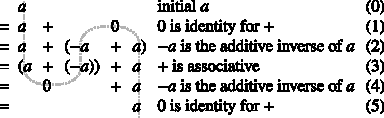
\includegraphics{diagrams/thesis/algebra-wire1.pdf}
}
\end{center}
Although seemingly pointless, this algebraic proof corresponds, in our model,
to an isomorphism of type {{a <-> a}} with a non-trivial and interesting
computational interpretation. The witness for this isomorphism is a
computation that takes a value of type~{{a}}, say \$20.00, and eventually
produces another \$20.00 value as its output. As the semantics of
Sec.~\ref{sec:rat} formalizes, this computation flows along the dotted line
with the following intermediate steps:
\begin{itemize}
\item We start at line (0) with \$20.00; 
\item We proceed to line (1) with the same \$20.00 but tagged as being
  in the left summand of the sum type {{a+0}}; we indicate this value
  as {{left 20}};
\item We continue to line (2) with the same value {{left 20}};
\item At line (3), as a result of re-association the tag on the \$20.00
  changes to indicate that it is in the left-left summand, i.e., the value is
  now {{left (left 20)}};
\item At line (4), we find ourselves needing to produce a value of type 0
  which is impossible; this signals the beginning of a reverse execution
  which sends us back to line (3) with a value {{left (right 20)}};
\item Execution continues in reverse to line (2) with the value 
  {{right (left 20)}};
\item At line (1) we find ourselves again facing an empty type so we reverse
  execution again; we go to line (2) with a value {{right (right 20)}};
\item We proceed to line (3) and (4) with the value {{right 20}};
\item We finally reach line 5 with the value {{20}}.
\end{itemize}
The example illustrates that the empty type and negative types have a
computational interpretation related to continuations: negative types denote
values that backtrack to satisfy dependencies, or in other words act as debts
that are satisfied by the backward flow of information.

\paragraph*{Fractional Types.} 
Consider a similar algebraic manipulation involving fractional types.
\begin{center}
\scalebox{1.1}{
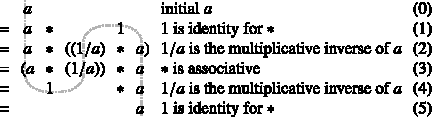
\includegraphics{diagrams/thesis/algebra-wire2.pdf}
}
\end{center}
In the case of negatives, the dotted line indicated the flow of control
whereas for fractionals it indicates the flow of constraints. At the heart of
logic programming is the idea of variables that capture constraints. Hence it
is useful to trace the computation corresponding to the algebraic proof
above, with the analogy to logic variables in mind.

As before, the execution begins at line~(0) with the value {{20}}. At
line~(1) two values, {{20}} and {{()}}, flow forward. One can think of the
value {{()}} (of type {{1}}) as ``having a credit card.'' The credit card
isn't money, nor is it debt, but is the option to generate a credit-debt
constraint.  At line~(2) we exercise this option and hence have three values:
the initial value {{20}} flowing from line (1) and two entangled values,
{{1/alpha}} and {{alpha}}. The {{alpha}} and {{1/alpha}} are unspecified
values, i.e., we don't yet know how much money we need to borrow, but we do
know that what is borrowed must be what is returned. Hence~{{alpha}} denotes
the presence of an unknown quantity and dually {{1/alpha}} should be thought
of as the absence of an unknown quantity. At line (3), the missing unknown
{{1/alpha}} is brought together with a value {{20}} and at line (4) we use
the {{20}} to satisfy the constraint {{1/alpha}}. In other words, this branch
of the computation succeeded in borrowing {{20}} which immediately
communicates the {{20}} to the rightmost branch.

Unlike with negative types, wherein only one value existed at a time and the
computation backtracked, here we have three values that \emph{exist at the
  same time}. In other words, the computation with fractions is realized with
a schedule in which every value independently and concurrently proceeds
through its subcomputation. The example illustrates that fractional types
also have a computational interpretation that have some flavor of
continuations: the fractional types denote values ({{1/alpha}}) that
represent missing information that must be supplied in much the same sense
that continuations denote evaluation contexts with holes that must be filled.

There are at least four fundamental points about the examples above that must
be emphasized:

\begin{itemize}
\item As the examples illustrate, both negative types and fractional types
  corresponds to ``debts'' but in different ways: negatives are satisfied by
  backtracking and fractionals are satisfied by constraint propagation.

\item It would clearly be disastrous if debts could be deleted or
  duplicated. This simple observation explains why these types are much
  simpler and much more appealing in a framework where information is
  guaranteed to be preserved. In previous work that used negative types (see
  Sec.~\ref{sec:related}), complicated mechanisms are typically needed to
  constrain the propagation and use of negative values because the
  surrounding computational framework is, generally speaking, careless in its
  treatment of information.

\item Each of the values {{-a + b}} and {{(1/a) * b}} can be viewed as a
  function that asks for an {{a}} and then produces a {{b}}. When viewed as
  functions, we write these types as {{a -o+ b}} and {{a -o* b}}
  respectively. Alternatively we can view these values as first producing a
  value of type {{b}} and then demanding an {{a}} and in that perspective
  they correspond to delimited continuations. Evidently, as the discussion
  above suggests, these two notions of functions are not the same at all and
  should not be conflated. Sec.~\ref{sub:hof} discusses this point in detail.

\item The main reason credit card transactions are convenient is because they
  disentangle the propagation of the resources (money) from the propagation
  of the services. Not every transaction needs both the resources and
  services to be brought together: it is sufficient to have a promise that
  the demand for resources will be somehow satisfied, as long as the
  infrastructure can be trusted with such promises. This idea that
  dependencies can be freely decoupled and propagated can be a powerful
  programming tool and we leverage this in the construction of a novel
  SAT-solver (see Sec.~\ref{sec:sat-solver}).
\end{itemize}

\paragraph*{Contributions and Outline.} 
To summarize, in a computational framework that guarantees that information
is preserved, negative and fractional types provide fascinating mechanisms in
which computations can be sliced and diced, decomposed and recomposed, run
forwards and backwards, in arbitrary ways. The remainder of the paper
formalizes these informal observations. Specifically our main contributions
are:
\begin{itemize}
\item We extend {{Pi}} our reversible programming language of type
  isomorphisms~\cite{rc2011,infeffects} (reviewed in Sec.~\ref{sec:pi}) with a notion
  of negative types, that satisfies the isomorphism {{a + (-a) <-> 0}}. The
  semantics of this extension is expressed by having a \emph{dual} evaluator
  that reverses the flow of execution for negative
  values. (Sec.~\ref{sec:neg})
\item We independently extend {{Pi}} with a notion of fractional types,
  that satisfies the isomorphism {{a * (1/a) <-> 1}}. The semantics of this
  extension is expressed by introducing logic variables and a unification
  mechanism to model and resolve the constraints introduced by the fractional
  types. (Sec.~\ref{sec:frac})
\item We combine the above two extensions into a language, which we
  call {{PiEE}}, whose type system allows any rational number to
  be used as a type. Moreover the types satisfy the same familiar and
  intuitive isomorphisms that are satisfied in the mathematical field
  of rational numbers. (Sec.~\ref{sec:rat})
\item We develop programming intuition and argue that negative and fractional
  types ought to be part of the vocabulary of every
  programmer. (Sec.~\ref{sec:prog})
\item We relate our notions of negative and fractional types to previous work
  on continuations. Briefly, we argue that conventional continuations
  conflate negative and fractional components. This observation allows us to
  relate two apparently unrelated lines of work: the first pioneered by
  Filinski~\cite{Filinski:1989:DCI:648332.755574} relating continuations to
  negative types and the second~\cite{Bernardi:2010:CSL:1749618.1749689}
  relating continuations to the fractional types of the Lambek-Grishin
  calculus. (Sec.~\ref{sec:related})
\end{itemize}

\textbf{Note:} All the constructions, semantics, and examples in this paper
have been implemented and tested in Haskell. We will make the URL available
once the code is organized for better presentation.

\end{comment}


%%%%%%%%%%%%%%%%%%%%%%%%%%%%%%%%%%%%%%%%%%%%%%%%%%%%%%%%%%%%%%%%%%%%%%%%%%%%%%%%
\section{The Core Reversible Language: {{Pi}} }
\label{sec:pi}

We review our reversible language {{Pi}}: the presentation in this
section differs from the one in our previous paper~\cite{infeffects} in two
aspects. First, we add the empty type {{0}} which is necessary to express the
additive duality. Second, instead of explaining evaluation using a natural
semantics, we give a small-step operational semantics that is more
appropriate for the connections with continuations explored in this paper.

%%%%%%%%%%%%%%%%%%%%
\subsection{Syntax and Types} 
\label{sec:pi-syntax}

The set of types includes the empty type {{0}}, the unit type {{1}}, sum
types {{b1+b2}}, and products types {{b1*b2}}. The set of values {{v}}
includes {{()}} which is the only value of type {{1}}, {{left v}} and {{right v}} 
which inject {{v}} into a sum type, and {{(v1,v2)}} which builds a
value of product type. There are no values of type {{0}}:
%subcode{bnf} include main
% value types, b ::= 0 | 1 | b + b | b * b 
% values, v ::= () | left v | right v | (v, v)

The combinators of {{Pi}} are witnesses to the following type
isomorphisms: 
%subcode{bnf} include main
%! columnStyle = r@{\hspace{-0.5pt}}c@{\hspace{-0.5pt}}l
%zeroe :&  0 + b <-> b &: zeroi
%swap+ :&  b1 + b2 <-> b2 + b1 &: swap+
%assocl+ :&  b1 + (b2 + b3) <-> (b1 + b2) + b3 &: assocr+
%identl* :&  1 * b <-> b &: identr*
%swap* :&  b1 * b2 <-> b2 * b1 &: swap*
%assocl* :&  b1 * (b2 * b3) <-> (b1 * b2) * b3 &: assocr*
%dist0 :& 0 * b <-> 0 &: factor0
%dist :&~ (b1 + b2) * b3 <-> (b1 * b3) + (b2 * b3)~ &: factor
Each line of the above table introduces one or two combinators that witness
the isomorphism in the middle. Collectively the isomorphisms state that the
structure {{(b,+,0,*,1)}} is a \emph{commutative semiring}, i.e., that each
of {{(b,+,0)}} and {{(b,*,1)}} is a commutative monoid and that
multiplication distributes over addition. The isomorphisms are extended to
form a congruence relation by adding the following constructors that witness
equivalence and compatible closure:
%subcode{proof} include main
%@  ~
%@@ id : b <-> b 
%
%@ c : b1 <-> b2
%@@ sym c : b2 <-> b1
%
%@ c1 : b1 <-> b2
%@ c2 : b2 <-> b3
%@@ c1(;)c2 : b1 <-> b3
%---
%@ c1 : b1 <-> b3
%@ c2 : b2 <-> b4
%@@ c1 (+) c2 : b1 + b2 <-> b3 + b4
%
%@ c1 : b1 <-> b3
%@ c2 : b2 <-> b4
%@@ c1 (*) c2 : b1 * b2 <-> b3 * b4

To summarize, the syntax of {{Pi}} is given as follows. 

\begin{definition}{(Syntax of {{Pi}})}
\label{def:Pi}
We collect our types, values, and combinators, to get the full language
definition.
%subcode{bnf} include main
% value types, b ::= 0 | 1 | b+b | b*b 
% values, v ::= () | left v | right v | (v,v) 
%
% comb.~types, t ::= b <-> b
% iso ::= zeroe | zeroi 
%     &|& swap+ | assocl+ | assocr+ 
%     &|& identl* | identr* 
%     &|& swap* | assocl* | assocr* 
%     &|& dist0 | factor0 | dist | factor 
% comb., c ::= iso | id | sym c | c (;) c | c (+) c | c (*) c 
\end{definition}

\paragraph*{Adjoint.} 
An important property of the language is that every combinator {{c}} has an
adjoint {{c{dagger}}} that reverses the action of {{c}}. This is evident by
construction for the primitive isomorphisms. For the closure combinators, the
adjoint is homomorphic except for the case of sequencing in which the order
is reversed, i.e., {{(c1 (;) c2){dagger} = (c2{dagger}) (;) (c1{dagger}) }}.

%%%%%%%%%%%%%%%
\subsection{Graphical Language}

The syntactic notation above is often obscure and hard to read.  Following
the tradition established for monoidal
categories~\cite{springerlink:10.1007/978-3-642-12821-94}, we present a
graphical language that conveys the intuitive semantics of the language
(which is formalized in the next section).

The general idea of the graphical notation is that combinators are modeled by
``wiring diagrams'' or ``circuits'' and that values are modeled as
``particles'' or ``waves'' that may appear on the wires. Evaluation therefore
is modeled by the flow of waves and particles along the wires.

%% In fact, when talking about {{Pi}} circuits, we will often use the
%% words {{value}} and {{particle}} interchangeably.

\begin{itemize}
\item The simplest sort of diagram is the {{id : b <-> b}} combinator which
  is simply represented as a wire labeled by its type {{b}}, as shown on the
  left. In more complex diagrams, if the type of a wire is obvious from the
  context, it may be omitted. When tracing a computation, one might imagine a
  value {{v}} of type {{b}} on the wire, as shown on the right.

  \begin{multicols}{2}
\begin{center}
\scalebox{0.95}{
%%subcode-line{pdfimage}[diagrams/thesis/b-wire.pdf]

\includegraphics{diagrams/thesis/b-wire.pdf}
}
\end{center}
\begin{center}
\scalebox{0.95}{
%%subcode-line{pdfimage}[diagrams/thesis/b-wire.pdf]

\includegraphics{diagrams/thesis/b-wire-value.pdf}
}
\end{center}
  \end{multicols}

\item The product type {{b1*b2}} may be represented using either one wire
  labeled {{b1*b2}} or two parallel wires labeled {{b1}} and {{b2}}. In the
  case of products represented by a pair of wires, when tracing execution
  using particles, one should think of one particle on each wire or
  alternatively as in folklore in the literature on monoidal categories as a
  ``wave.''
\begin{multicols}{2}
\begin{center}
\scalebox{0.95}{
%%subcode-line{pdfimage}[diagrams/thesis/pair-one-wire.pdf]

\includegraphics{diagrams/thesis/product-one-wire.pdf}
}
\end{center}
\begin{center}
\scalebox{0.95}{

\includegraphics{diagrams/thesis/product-one-wire-value.pdf}
}
\end{center}
\end{multicols}
\begin{multicols}{2}
\begin{center}
\scalebox{0.95}{
%%%subcode-line{pdfimage}[diagrams/thesis/pair-of-wires.pdf]
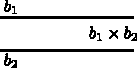
\includegraphics{diagrams/thesis/product-two-wires.pdf}
}
\end{center}
\begin{center}
\scalebox{0.95}{
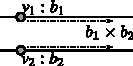
\includegraphics{diagrams/thesis/product-two-wires-value.pdf}
}
\end{center}
\end{multicols}

\item Sum types may similarly be represented by one wire or using
  parallel wires with a {{+}} operator between them. When tracing the
  execution of two additive wires, a value can reside on only one of the two
  wires.
\begin{multicols}{2}
\begin{center}
\scalebox{0.95}{
%%subcode-line{pdfimage}[diagrams/thesis/sum-one-wire.pdf]

\includegraphics{diagrams/thesis/sum-one-wire.pdf}
}
\end{center}
\begin{center}
\scalebox{0.95}{
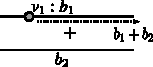
\includegraphics{diagrams/thesis/sum-two-wires-left-value.pdf}
}
\end{center}
\end{multicols}
\begin{multicols}{2}
\begin{center}
\scalebox{0.95}{
%%subcode-line{pdfimage}[diagrams/thesis/sum-of-wires.pdf]
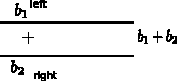
\includegraphics{diagrams/thesis/sum-two-wires.pdf}
}
\end{center}
\begin{center}
\scalebox{0.95}{
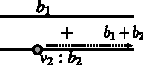
\includegraphics{diagrams/thesis/sum-two-wires-right-value.pdf}
}
\end{center}
\end{multicols}


%% \item
%% When representing complex types like {{(b1*b2)+b3}} some visual
%% grouping of the wires may be done to aid readability. The exact type
%% however will always be clarified by the context of the diagram.

%% \begin{center}
%% \scalebox{0.95}{
%% %subcode-line{pdfimage}[diagrams/thesis/complex-type-crop.pdf]
%% }
%% \end{center}

\item Associativity is implicit in the graphical language. Three parallel
  wires represent {{b1*(b2*b3)}} or {{(b1*b2)*b3}}, based on the context.
\begin{center}
\scalebox{0.95}{
%%subcode-line{pdfimage}[diagrams/thesis/associate.pdf]
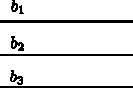
\includegraphics{diagrams/thesis/assoc.pdf}
}
\end{center}

\item Commutativity is represented by crisscrossing wires.
\begin{multicols}{2}
\begin{center}
\scalebox{0.95}{
%%subcode-line{pdfimage}[diagrams/thesis/swap-pair.pdf]
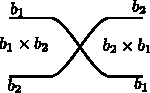
\includegraphics{diagrams/thesis/swap_times.pdf}
}
\end{center}
\begin{center}
\scalebox{0.95}{
%%subcode-line{pdfimage}[diagrams/thesis/swap-sum.pdf]
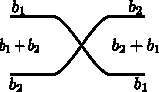
\includegraphics{diagrams/thesis/swap_plus.pdf}
}
\end{center}
\end{multicols}

By visually tracking the flow of particles on the wires, one can
verify that the expected types for commutativity are satisfied.

\begin{multicols}{2}
\begin{center}
\scalebox{0.95}{
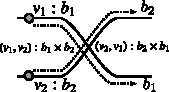
\includegraphics{diagrams/thesis/swap_times_value.pdf}
}
\end{center}
\begin{center}
\scalebox{0.95}{
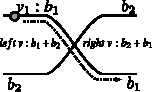
\includegraphics{diagrams/thesis/swap_plus_value.pdf}
}
\end{center}
\end{multicols}


\item The morphisms that witness that {{0}} and {{1}} are the additive and
  multiplicative units are represented as shown below. Note that since there
  is no value of type 0, there can be no particle on a wire of type {{0}}.
  Also since the monoidal units can be freely introduced and eliminated, in
  many diagrams they are omitted and dealt with explicitly only when they are
  of special interest.
\begin{multicols}{2}
\begin{center}
\scalebox{0.95}{
%%subcode-line{pdfimage}[diagrams/thesis/identr1.pdf]
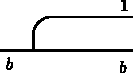
\includegraphics{diagrams/thesis/uniti.pdf}
}
\end{center}
\begin{center}
\scalebox{0.95}{
%%subcode-line{pdfimage}[diagrams/thesis/identl1.pdf]
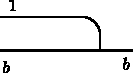
\includegraphics{diagrams/thesis/unite.pdf}
}
\end{center}  
\end{multicols}
\begin{multicols}{2}
\begin{center}
\scalebox{0.95}{
%%subcode-line{pdfimage}[diagrams/thesis/identr0.pdf]
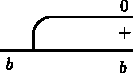
\includegraphics{diagrams/thesis/zeroi.pdf}
}
\end{center}
\columnbreak
\begin{center}
\scalebox{0.95}{
%%subcode-line{pdfimage}[diagrams/thesis/identl0.pdf]
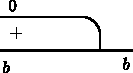
\includegraphics{diagrams/thesis/zeroe.pdf}
}
\end{center}
\end{multicols}

\item Finally, distributivity and factoring are represented using the dual
  boxes shown below:
\begin{multicols}{2}
\begin{center}
  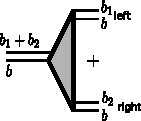
\includegraphics{diagrams/thesis/dist.pdf}
\end{center}
\begin{center}
  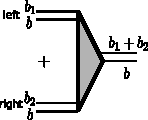
\includegraphics{diagrams/thesis/factor.pdf}
\end{center}
\end{multicols}


Distributivity and factoring are interesting because they represent
interactions between sum and pair types. Distributivity should
essentially be thought of as a multiplexer that redirects the flow of
{{v:b}} depending on what value inhabits the type {{b1+b2}}, as shown
below. Factoring is the corresponding adjoint operation.

\begin{multicols}{2}
\begin{center}
  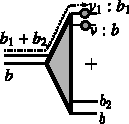
\includegraphics{diagrams/thesis/dist-wire-value1.pdf}
\end{center}
\begin{center}
  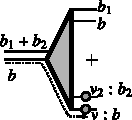
\includegraphics{diagrams/thesis/dist-wire-value2.pdf}
\end{center}
\end{multicols}


\end{itemize}

\noindent 
\textit{Example.}  We use the type {{bool}} as a shorthand to denote
the type {{1+1}} and use {{left ()}} to be {{true}} and {{right ()}}
to be {{false}}. The following combinator is represented by the given
diagram:

{{c : b * bool <-> b + b}}

{{c = swap* (;) dist (;) (identl* (+) identl*)}}

\begin{center}
\scalebox{0.95}{
%%subcode-line{pdfimage}[diagrams/thesis/example1-crop.pdf]
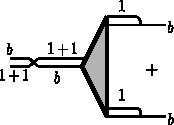
\includegraphics{diagrams/thesis/example1.pdf}
}
\end{center}

%%%%%%%%%%%%%%%%%%%%%%%
\subsection{Semantics}

The semantics of the primitive combinators is given by the following
single-step reductions. Since there are no values of type {{0}}, the rules
omit the impossible cases:
\begin{scriptsize}
%subcode{opsem} include main
%! columnStyle = rlcl
% swap+ & (left v) &|-->& right v
% swap+ & (right v) &|-->& left v 
% assocl+ & (left v1) &|-->& left (left v1)
% assocl+ & (right (left v2)) &|-->& left (right v2)
% assocl+ & (right (right v3)) &|-->& right v3 
% assocr+ & (left (left v1)) &|-->& left v1
% assocr+ & (left (right v2)) &|-->& right (left v2)
% assocr+ & (right v3) &|-->& right (right v3)
% identl* & ((), v) &|-->& v 
% identr* & v &|-->& ((), v) 
% swap* & (v1, v2) &|-->& (v2, v1) 
% assocl* & (v1, (v2, v3)) &|-->& ((v1, v2), v3) 
% assocr* & ((v1, v2), v3) &|-->& (v1, (v2, v3)) 
% dist & (left v1, v3) &|-->& left (v1, v3)
% dist & (right v2, v3) &|-->& right (v2, v3)
% factor & (left (v1, v3)) &|-->& (left v1, v3) 
% factor & (right (v2, v3)) &|-->& (right v2, v3)   

%subcode{proof} include main
%@ ~
%@@ id v |--> v 
%
%@ c{dagger} v1 |--> v2
%@@ (sym c) v1 |--> v2
%
%@ c1  v1 |--> v
%@ c2  v |--> v2
%@@ (c1(;)c2)  v1 |--> v2
%---
%@ c1  v1 |--> v2
%@@ (c1 (+) c2)  (left v1) |--> left v2
%
%@ c2  v1 |--> v2
%@@ (c1 (+) c2)  (right v1) |--> right v2
%---
%@ c1  v1 |--> v3
%@ c2  v2 |--> v4
%@@ (c1 (*) c2)  (v1, v2) |--> (v3, v4)
\end{scriptsize}

\begin{proposition}[Type Safety]
  
\end{proposition}

\begin{proposition}[Strong Normalizing]
\label{prop:termination-pi} 
{{Pi}} computation always terminate.  

{{forall. c:b1<->b2, v:b1, exists v':b2.}}  
{{c v |--> v'}}
\end{proposition}

\begin{proposition}[Logical Reversibility]
\label{prop:logrev}
{{c v |--> v'}} iff 
{{ c{dagger} v' |--> v}}
\end{proposition}

\subsection{Small Step Semantics}

The reductions for the primitive isomorphisms above are exactly the same as
have been presented before~\cite{infeffects}. The reductions for the closure
combinators are however presented in a small-step operational style using the
following definitions of evaluation contexts and machine states:

\begin{scriptsize}
%subcode{bnf} include main
% Combinator Contexts, C = [] | Fst C c | Snd c C 
%                  &|& LeftT C c v | RightT c v C 
%                  &|& LeftP C c | RightP c C 
% Machine states = <c, v, C> | {[c, v, C]}
% Start state = <c, v, []> 
% Stop State = {[c, v, []]}
\end{scriptsize}
The machine transitions below track the flow of particles through a
circuit. The start machine state, , denotes the
particle~{{v}} about to be evaluated by the circuit {{c}}. The end
machine state, {{[c, v, [] ]}}, denotes the situation where the particle
{{v}} has exited the circuit {{c}}.

\begin{scriptsize}
%subcode{opsem} include main
%! columnStyle = rclr
% <iso, v, C> &|-->& {[iso, v', C]} & (1)
% & & where iso v |--> v' &
% <c1(;)c2, v, C> &|-->& <c1, v, Fst C c2> & (2) 
% {[c1, v, Fst C c2]} &|-->& <c2, v, Snd c1 C> & (3) 
% {[c2, v, Snd c1 C]} &|-->& {[ c1(;)c2, v, C ]} & (4) 
% <c1(+)c2, left v, C> &|-->& <c1, v, LeftP C c2> & (5) 
% {[ c1, v, LeftP C c2 ]} &|-->& {[c1 (+) c2, left v, C ]} & (6)
% <c1(+)c2, right v, C> &|-->& <c2, v, RightP c1 C> & (7)
% {[ c2, v, RightP c1 C ]} &|-->& {[c1 (+) c2, right v, C ]} & (8)
% <c1(*)c2, (v1, v2), C> &|-->& <c1, v1, LeftT C c2 v2> & (9)
% {[ c1, v1, LeftT C c2 v2 ]} &|-->& <c2, v2, RightT c1 v1 C> & (10) 
% {[ c2, v2, RightT c1 v1 C ]} &|-->& {[ c1 (*) c2, (v1, v2), C ]} & (11)
\end{scriptsize}
Rule (1) describes evaluation by a primitive isomorphism. Rules (2), (3) and
(4) deal with sequential evaluation. Rule (2) says that for the value {{v}}
to flow through the sequence {{c1 (;) c2}}, it should first flow through
{{c1}} with {{c2}} pending in the context ({{Fst C c2}}). Rule (3) says the
value {{v}} that exits from {{c1}} should proceed to flow
through~{{c2}}. Rule (4) says that when the value {{v}} exits {{c2}}, it also
exits the sequential composition {{c1(;)c2}}. Rules (5) to (8) deal with 
{{c1 (+) c2}} in the same way. In the case of sums, the shape of the value,
i.e., whether it is tagged with {{left}} or {{right}}, determines whether
path {{c1}} or path {{c2}} is taken. Rules (9), (10) and (11) deal with 
{{c1 (*) c2}} similarly. In the case of products the value should have the
form {{(v1, v2)}} where {{v1}} flows through {{c1}} and {{v2}} flows through
{{c2}}. Both these paths are entirely independent of each other and we could
evaluate either first, or evaluate both in parallel. In this presentation we
have chosen to follow {{c1}} first, but this choice is entirely arbitrary.

The interesting thing about the semantics is that it represents a reversible
abstract machine. In other words, we can compute the start state from the
stop state by changing the reductions {{|-->}} to run backwards
{{<--|}}. When running backwards, we use the isomorphism represented by a
combinator {{c}} in the reverse direction, i.e., we use the adjoint
{{c{dagger}}}.

\begin{proposition}[Correspondence]
  Evaluation in the small-step evaluator corresponds to evaluation in
  the natural semantics.

  {{c v |--> v'}} iff {{<c, v, []> |-->* [c, v', [] ]}}

\end{proposition}

Consequently the small step semantics is logically reversible and
strong normalizing. 

\begin{proposition}[Type Safety]
  
\end{proposition}


% \roshan{We really have to rethink this prop in the presence of
%   negatives and fractionals. With negatives, the program can actually
%   end at the beginning of the circuit -- i.e. the program {{c:b1<->b2}}
%   can stop with a value of type {{b1}}. With fractionals, there can be
%   several values of type {{b2}} produced for a value of type {{b1}}. }

% \begin{proposition}[Groupoid]
% \label{prop:groupoid}
% {{Pi}} is a groupoid. 
% \end{proposition}

% \begin{proposition}
% \label{prop:category}
% {{Pi}} is a dagger symmetric monoidal category. 
% \end{proposition}

%%%%%%%%%%%%%%%%%%%%%%%%%%%%%%%%%%%%%%%%%%%%%%%%%%%%%%%%%%%%%%%%%%%%%%%%%%%%%%%%
% \section{First class functions from the permutation space.}

%%%%%%%%%%%%%%%%%%%%%%%%%%%%%%%%%%%%%%%%%%%%%%%%%%%%%%%%%%%%%%%%%%%%%%%%%%%%%%%%
\section{Traces and the Int-Construction.}

For a traced symmetric monoidal category, the Int-construction of
Joyal, Street and Verity \cite{joyal1996traced} gives us a way of
constructing a compact closed category. This is the obvious first
thing to try for a duality in this setting.

%subcode{proof} include main
%@ c : b1 + b2 <-> b1 + b3
%@@ trace c : b2 <-> b3  

%% \begin{center}
%%   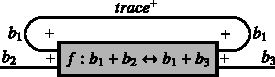
\includegraphics{diagrams/thesis/trace_plus.pdf}
%% \end{center}

Show that the int construction does not preserve the {{*}} tensor. We
need a duality that preserves both tensors.

%%%%%%%%%%%%%%%%%%%%%%%%%%%%%%%%%%%%%%%%%%%%%%%%%%%%%%%%%%%%%%%%%%%%%%%%%%%%%%%%
\section{Fractional Types : {{PiEE*}} }

%subcode{bnf} include main
% Value Types, b = 0 | 1 | b + b | b * b  | 1/b
% Values, v = () | left v | right v | (v, v) | 1/v
%
% Isomorphisms, iso &=& ... | eta* | eps*

\noindent
No division by zero. 

\begin{multicols}{2}  
%subcode{opsem} include main
% eta* &: 1 <-> (1/b) * b :& eps*

%subcode{proof} include main
%@ |- v : b
%@@ |- 1/v : 1/b
\end{multicols}

For the graphical language, we visually represent {{eta*}}, and
{{eps*}} as U-shaped connectors. On the left below is {{eta*}} showing
the map and {{1}} to {{1/b * b}}.  On the right is {{eps*}} showing
the map from {{1/b * b}} to~1. Even though the diagrams below show the
{{1}} wires for completeness, later diagrams will always drop them in
contexts where they can be implicitly introduced and eliminated.
\begin{multicols}{2}
\begin{center}
  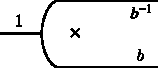
\includegraphics{diagrams/eta_times.pdf}
\end{center}
  
\begin{center}
  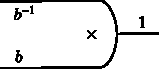
\includegraphics{diagrams/eps_times.pdf}
\end{center}
\end{multicols}

The usual interpretation of {{b1*b2}} we have both a value of type
{{b1}} and a value of type {{b2}}. This interpretation is maintained
in the presence of fractionals. Hence an {{eta* : 1 <-> (1/b) * b}} is
to be viewed as a fission point for a value of type {{b}} and its
multiplicative inverse {{1/b}}. Operationally, this corresponds to the
creation of two values {{alpha}} and {{1/alpha}} where {{alpha}} is a
fresh logic variable. The operator {{eps*}} then becomes a unification
site for these logic variables:

\begin{multicols}{2}
\begin{center}
\scalebox{1.5}{
  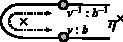
\includegraphics{diagrams/eta_times1.pdf}
}
\end{center}

\begin{center}
\scalebox{1.5}{
  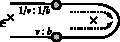
\includegraphics{diagrams/eps_times1.pdf}
}
\end{center}  
\end{multicols}

Negative Information and Measurements. 

Compact Closed Structure (modulo 0). 

Show that ``no division by zero'' is supported by the semantics. 

%%%%%%%%%%%%%%%%%%%%%%%%%%%%%%%%%%%%%%%%%%%%%%%%%%%%%%%%%%%%%%%%%%%%%%%%%%%%%%%%
\subsection{Semantics}

Provide a semantics with the non-determinism monad and define an
\emph{eval}.

\begin{proposition}[Type Safety]
  
\end{proposition}

\begin{proposition}[Strong Normalizing]
  
\end{proposition}

Note that this language is not logically reversible. 

For a monoidal category to be compact closed the maps~{{eta}}
and~{{eps}} must satisfy a coherence condition that is usually
visualized as follows:
\begin{center}
  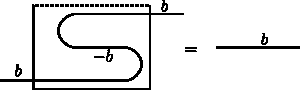
\includegraphics{diagrams/coherence.pdf}
\end{center}
where $b^*$ represents the dual of {{b}}.  In the case of negatives,
the condition amounts to checking that reversing direction twice is a
no-op. In the case of fractionals, the condition amounts to checking
that creating values {{alpha}} and {{1/alpha}} and immediately
unifying them is also a no-op. Both checks are straightforward and are
essentially the constructions in the introduction.

\begin{proposition}[Coherence]
  
\end{proposition}


%%%%%%%%%%%%%%%%%%%%
\subsection{Categorical Constructions}

All the constructions below are standard: they are collected from Selinger's
survey paper on monoidal
categories~\cite{springerlink:10.1007/978-3-642-12821-94} and presented in
the context of our language. 

We now review several interesting constructions related to looping,
involution, and higher order functions. 

\paragraph*{Trace.}
Every compact closed category admits a trace. For the additive case, we get
the following definition.  Given {{f : b1+b2 <-> b1+b3 }}, 
define {{trace+ f : b2 <-> b3}} as:

{{ trace+ f = zeroi (;) (id (+) eta+) (;) (f (+) id) (;) (id (+) eps+) (;) zeroe }} 

\begin{center}
  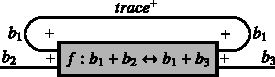
\includegraphics{diagrams/thesis/trace_plus.pdf}
\end{center}  

\noindent We have omitted some of the commutativity and associativity
shuffling to communicate the main idea. We are given a value of type
{{b2}} which we embed into {{0+b2}} and then {{(-b1+b1)+b2)}}. This
can be re-associated into {{-b1+(b1+b2)}}. The component {{b1+b2}},
which until now is just an appropriately tagged value of type {{b2}},
is transformed to a value of type {{b1+b3}} by {{f}}. 
If the result is in the {{b3}}-summand, it is produced as
the answer; otherwise the result is in the {{b1}}-summand; {{eps+}} is
used to make it flow backwards to be fed to the {{eta+}} located at
the beginning of the sequence. Iteration continues until a {{b3}} is
produced.


%%%%%
\paragraph*{Involution (Principium Contradictiones)}

In a symmetric compact closed category, we can build isomorphisms that the
dual operation is an involution. Specifically, we get the isomorphisms 
{{b <-> -(-b)}} and {{b <-> (1/(1/b))}}. For the additive case, the 
isomorphism is defined as follows:

{{ (id (+) eta+) (;) (swap+ (+) id) (;) (id (+) eps+) }}

\noindent where we have omitted the 0 introduction and elimination. The idea
is as follows: we start with a value of type {{b}}, embed it into {{b+0}} and
use {{eta}} to create something of type {{b + (-(-b) + (-b))}}. This is possible
because {{eta}} has the polymorphic type {{-a + a}} which can be instantiated
to {{-b}}. We then reshuffle the type to produce {{-(-b) + (-b + b)}} and cancel
the right hand side using {{eps+}}.  The construction for the multiplicative 
case is identical and omitted.

%% {{b <-> -(-b)}}
%% 
%% this is the wrong diagram: see lemma 4.17 in selinger's paper
%% \begin{center}
%%   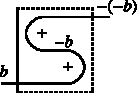
\includegraphics{diagrams/double_neg.pdf}
%% \end{center}

\paragraph*{Duality preserves the monoidal tensor. }
As with compact closed categories, the dual on the objects distributes
over the tensor. In terms of {{PiEE}} we have that {{-(b1+b2)}}
can be mapped to {{(-b1)+(-b2)}} and that {{1/(b1*b2)}} can be mapped
to {{(1/b1)*(1/b2)}}. The isomorphism {{-(b1 + b2) <-> (-b1) + (-b2)}}
can be realized as follows:
\begin{center}
  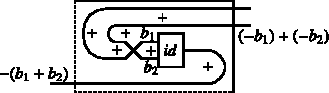
\includegraphics{diagrams/dist_neg_plus.pdf}
\end{center}

\noindent
The multiplicative construction is similar. 

%% This is a distinguishing difference from *-autonomous categories that
%% are models for Linear Logic, where the dual does not preserve the
%% tensor but maps to a dual tensor \cite{curien2009interactive}.

\paragraph*{Duality is a functor.}
Duality in {{PiEE}} can map objects to their duals and morphisms
to act on dual objects. In other {{c : b1 <-> b2}} to
{{neg~c:-b1<->-b2}} in the additive monoid and to
{{inv~c:1/b1<->1/b2}} in the multiplicative monoid. 
%% Any operation on types can be applied to the negative versions of these
%% types. 
The idea is simply to reverse the flow of values and use the
adjoint of the operation:
\begin{multicols}{2}
\begin{center}
  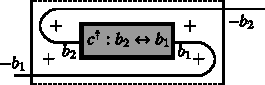
\includegraphics{diagrams/neg_lift.pdf}
\end{center}  

%subcode{proof} include main
%@ c : b1 <-> b2
%@@ neg c : (-b1) <-> (-b2)
\end{multicols}

This construction relies on the fact that every {{PiEE}} morphism
has an adjoint.  The {{inv}} construction is similar.

%% inverse morphism, whereas in compact closed categories with no
%% underlying dagger structure we can only construct an op-functor.


%%%%%%%%%%%%%%%%%%%%%%%%%%%%%%%%%%%%%%%%%%%%%%%%%%%%%%%%%%%%%%%%%%%%%%%%%%%%%%%%
\section{SAT Solver }
\label{sec:prog}
\label{sec:sat-solver}

% Additive traces correspond to iteration and multiplicative traces
% correspond to fixpoint of constraints. Addtive traces have been
% studied in the past \cite{infeffects} and here we focus on the
% multiplicative trace.

% The construction presented here is a novel SAT-solver that relies on
% {{trace*}} for its solution. It varies from previous classical SAT solvers
% \amr{must cite ???} in that there is no explicit search operation on the
% boolean space. It also varies from previous quantum SAT solvers \amr{must
%   cite ???} in that it does uses a {{trace}} operation to compute a fixpoint
% which is the solution following which an isomorphic clone operation allows us
% to examine the result.  Though we focus on SAT here, this construction can be
% generalized to any constraint satisfaction problem whose search space can be
% represented by a recursive type and for which an isomorphic clone operation
% can be constructed. 
% can be constructed. Before we start, let us recall two constructions:

We illustrate the expressive power of first-class constraints represented by
fractional types. To understand the intuition, recall the definition of
{{trace}} for the multiplicative fragment of {{PiEE}}. 
Given {{f : a*c <-> b*c }}, we have {{trace* f : a <-> b}}: 

{{ trace* f = uniti (;) (id (*) eta*) (;) (f (*) id) (;) (id (*) eps*) (;) unite }}

\noindent This circuit uses {{eta*}} to generate all possible {{c}}-values
together with an associated {{(1/c)}}-constraint. It then applies {{f}} to the
pair {{(a,c)}}. The function {{f}} must produce an output {{(b,c')}} for each
such input. If the input {{c}} and the output {{c'}} are the same they can be
annihilated by {{eps*}}; otherwise the execution gets stuck and this
particular choice of {{c}} is pruned. 

% Annihilation and non-termination describe undefined program
% execution. While non-termination characterizes an iteration that fails
% to terminate, annihilation characterizes a constraint that has no
% fixpoint. The SAT-solver of Sec. \ref{sec:sat-solver} works by
% annihilating only the program states that do not match the boolean
% satisfiability constraint.
% \emph{Annihilation.}  
% With {{eta*}} and {{eps*}}, we can construct a {{trace*}} operation
% which gives us the ability to find the fixpoint of a constraint.  If
% the constraint has no satisfying values, there is no fixpoint possible
% -- we use the term \emph{annihilation} to describe the corresponding
% undefined state of the program.

A large class of constraint satisfaction problems can be expressed
using {{trace*}}. We illustrate the main ideas with the implementation
of a SAT-solver.  We proceed in small steps, reviewing some of the
necessary constructions presented in our earlier
paper~\cite{infeffects}.

%%%%%%%%%%%%%%%%%%%
\subsection{Booleans and Conditionals} 

Given any combinator {{c : b <-> b}} we can construct a combinator called
{{if_c : bool*b <->bool*b}} in terms of {{c}}, where {{if_c}} behaves like a
one-armed $\mathit{if}$-expression. If the supplied boolean is {{true}} then
the combinator {{c}} is used to transform the value of type~{{b}}. If the
boolean is {{false}}, then the value of type {{b}} remains unchanged. We can
write down the combinator for {{if_c}} in terms of {{c}} as 
{{ dist (;) ((id (*) c) (+) id) (;) factor }}.

\noindent The diagram below shows the input value of type {{(1+1)*b}}
processed by the distribute operator {{dist}}, which converts it into a value
of type {{(1*b)+(1*b)}}. In the {{left}} branch, which corresponds to the
case when the boolean is {{true}} (i.e. the value was {{left ()}}), the
combinator~{{c}} is applied to the value of type~{{b}}. The right branch
which corresponds to the boolean being {{false}} passes along the value of
type {{b}} unchanged.

\begin{center}
\scalebox{1.0}{
%%subcode-line{pdfimage}[diagrams/if_c.pdf]
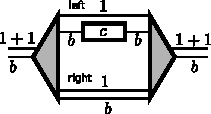
\includegraphics{diagrams/thesis/cnot.pdf}
}
\end{center}

% We will be seeing many more such wiring diagrams in this paper and it is
% useful to note some conventions about them. Wires indicate a
% value that can exist in the program. Each wire, whenever possible, is
% annotated with its type and sometimes additional information to help clarify
% its role. When multiple wires run in parallel, it means that those values
% exist in the system at the same time, indicating pair types. When there is a
% disjunction, we put a {{+}} between the wires. 
% Combinators for distribution {{dist}} and factoring {{factor}}
% are represented as triangles with their operator symbols in them. Other
% triangles may be used and, in each case, types or labels will be used to
% clarify their roles. Finally, we don't draw boxes for combinators such as
% {{id}}, commutativity, and associativity, but instead just shuffle the wires
% as appropriate.

The combinator {{if_{not} }} has type {{bool*bool<->bool*bool}} and
negates its second argument if the first argument is {{true}}. This
gate {{if_{not} }} is often referred to as the {{cnot}} gate. An
equivalent construction that is useful is {{else_{not} }} where we
negate the second argument only if the first is {{false}}. 

Similarly, we can iterate the construction of {{if_c}} to check several
bits. The gate {{if_{cnot} }}, which we may also write as {{if^2_{not} }},
checks two booleans and negates the result wire only if they are both
{{true}}. The gate {{if^2_{not} }} is well known as the Toffoli gate and is a
universal reversible gate. We can generalize this construction to
{{if^n_{not} }} which checks {{n}} bits and negates the result wire only if
they are all {{true}}.

%%%%%%%%%%%%%%%%%%
\subsection{Cloning}

Although cloning is generally not allowed in reversible languages, it is
possible at the cost of having additional constant inputs. For example,
consider the gate {{else_{not} }}. Generally, the gate maps
{{(false,a)}} to {{(false,not a)}} and {{(true,a)}} to {{(true,a)}}. Focusing
on the cases in which the second input is {{true}}, we get that the gate maps
{{(false,true)}} to {{(false,false)}} and {{(true,true)}} to {{(true,true)}},
i.e., the gate clones the first input. A circuit of {{n}} parallel
{{else_{not} }} gates can hence clone {{n}} bits.  They also consume {{n}}
{{true}} inputs in the process.  Let us call this construction
{{clone^n_{bool} }}.

%%%%%%%%%%%%%%%%%%%%%%%%%%%%%
\subsection{Construction of the Solver}

The key insight underlying the construction comes from the fact that we can
build \emph{annihilation circuits} such as the one below:

\begin{center}
\scalebox{1.2}{
  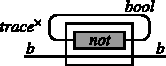
\includegraphics{diagrams/not_trace.pdf}
}
\end{center}
The circuit constructs a boolean {{b}} and its dual {{1/b}}, negates one of
them and attempts to satisfy the constraint that they are equal which
evidently fails. 

With a little work, we can modify this circuit to only annihilate values that
fail to satisfy the constraints represented by a SAT-instance {{f}}. In more
detail, an instance of SAT is a function/circuit~{{f}} that given some
boolean inputs returns {{true}} or {{false}} which we interpret as whether
the inputs satisfy the constraints imposed by the structure of {{f}}. Because
we are in a reversible world, our instance of SAT must be expressed as an
isomorphism: this is easily achieved as shown in Sec.~\ref{sub:f}
below. Assuming that {{f}} is expressed as an isomorphism, we have enough
information to reconstruct the input from the output. This can be done by
using the adjoint of {{f}}. At this point we have, the top half of the
construction below:

\begin{center}
\scalebox{1.2}{
  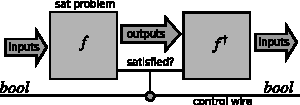
\includegraphics{diagrams/sat1.pdf}
}
\end{center}  

To summarize, the top half of the circuit is the identity function except
that we have also managed to produce a boolean wire labeled
\textsf{satisfied?} that tells us if the inputs satisfy the desired
constraints. We can take this boolean value and use it to decide whether to
negate the control wire or not. Thus, the circuit achieves the following
goal: if the inputs do not satisfy {{f}}, the control wire is negated.  We
can now use {{trace*}} to annihilate all these bad values because the control
wire acts like the closed-loop {{not}} in the previous construction.

%%%%%%%%%%%%%%%%%%%%%%%%%%%%%%%%%%%%%%%%%%%%%%%%%%%%%%%%%%%%%%%%%%%%%%%%
\subsection{Final Details}
\label{sub:f}

Any boolean expression {{f : bool^n -> bool}} can be compiled into the
isomorphism {{iso_f : bool^h*bool^n<->bool^g*bool}} where the extra bits
{{bool^h}} and {{bool^g}} are considered as heap and garbage. Constructing
such an isomorphism has been detailed
before~\cite{Toffoli:1980,infeffects}. The important relation to note is that
applying {{iso_f}} to some special heap values and an input \textit{bs}
produces some bits that can be ignored and the same output that {{f}} would
have produced on {{bs}}. We can ensure that the heap has the appropriate
initial values by checking the heap and negating a second control wire, if
the values do not match, i.e., the dotted part in the diagram below.

\begin{center}
\scalebox{1.2}{
  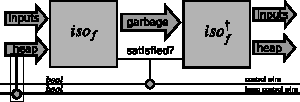
\includegraphics{diagrams/sat2.pdf}
}
\end{center}  

% \roshan{Explain how the dotted part is implemented.}

Let us call the above construction which maps inputs, heap, and
control wires to inputs, heap, and control wires as {{sat_f}}. The
SAT-solver is is completed by tracing the {{sat_f}} and cloning the
inputs using {{clone^n_{bool} }}.

\begin{center}
\scalebox{1.5}{
  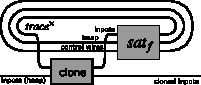
\includegraphics{diagrams/sat3.pdf}
}
\end{center}

When the solver is fed inputs initialized to {{true}}, it clones only
those inputs to {{sat_f}} that satisfy {{f}} and the heap
constraints. In the case of unique-SAT the solver will produce exactly
0 or 1 solutions. In the case of general SAT, the solver will produce
solutions as determined by the semantics of the top-level interaction
(see discussion in Sec. \ref{sec:rat}).


%%%%%%%%%%%%%%%%%%%%%%%%%%%%%%%%%%%%%%%%%%%%%%%%%%%%%%%%%%%%%%%%%%%%%%%%%%%%%%%%
\section{Finite Dimensional Hilbert Spaces}



Halmos \cite{halmos1958finite}, Abramsky and Coecke
\cite{abramsky2004categorical}. Despite the fact that this fragment
seem badly behaved (no logical reversibility) we have a close
connection with finite dimensional Hilbert spaces.

The technical goal of this section is to show that the categorical
structure of finite dimensional Hilbert spaces with unitary maps and
inner product has the same categorical structure as {{PiEE*}}. Thus
constructions in {{PiEE*}} can be transported to FdHilb-unitary. If we
allow all linear maps, then {{+}} becomes a biproduct.  This has
connections to the Quantum Picturisms of Abramsky and Coecke and hence
to Quantum Physics.

%subcode{bnf} include main
% v = 0 | 1 | v + v | v * v| 1/v 

There is much future work to be done in this line. The logical
consequence of this line of research is either (1) there is no way to
accommodate probabilities etc in this setting and this is all
meaningless or (2) constructions in {{PiEE*}} correspond to physical
phenomena.

Also show the what the irreversible constructions can be interpreted
in Dirac style.


%%%%%%%%%%%%%%%%%%%%%%%%%%%%%%%%%%%%%%%%%%%%%%%%%%%%%%%%%%%%%%%%%%%%%%%%%%%%%%%%
\section{Negative Types : {{PiEE+}} }

What is a negative type anyway? 


%subcode{bnf} include main
% Value Types, b = 0 | 1 | b + b | b * b | -b
% Values, v = () | left v | right v | (v, v) | -v 
%
% Isomorphisms, iso &=& ... | eta+ | eps+

For convenience, we sometimes use the notations {{b1 - b2}} and
{{b1/b2}} to indicate the types {{b1 + (-b2)}} and {{b1 * (1/b2)}}
respectively.  The types of the new constructs are:
\vspace{-15pt}
\begin{multicols}{2}  
%subcode{opsem} include main
% eta+ &: 0 <-> (-b) + b :& eps+

%subcode{proof} include main
%@ |- v : b
%@@ |- -v : -b
\end{multicols}


\begin{multicols}{2}
\begin{center}
  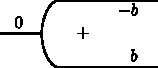
\includegraphics{diagrams/eta.pdf}
\end{center}
  
\begin{center}
 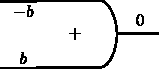
\includegraphics{diagrams/eps.pdf}
\end{center}
\end{multicols}

\begin{multicols}{2}
\begin{center}
\scalebox{1.5}{
  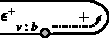
\includegraphics{diagrams/eps_plus1.pdf}
}
\end{center}
  
\begin{center}
\scalebox{1.5}{
  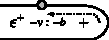
\includegraphics{diagrams/eps_plus2.pdf}
}
\end{center}  
\end{multicols}


%%%%%%%%%%%%%%%%%%%%%%%%%%%%%%%%%%%%%%%%%%%%%%%%%%%%%%%%%%%%%%%%%%%%%%%%%%%%%%%%
\subsection{Semantics}

%subcode{opsem} include main
%! columnStyle = rclr
%! fwd = \triangleright
% <iso, v, C, s>_{fwd} &|-->& {[iso, v', C, s']}_{fwd}
% & & where iso s v |--> (v', s')
% <c1(;)c2, v, C, s>_{fwd} &|-->& <c1, v, Fst C c2, s>_{fwd}
% {[c1, v, Fst C c2, s]}_{fwd} &|-->& <c2, v, Snd c1 C, s>_{fwd}
% {[c2, v, Snd c1 C, s]}_{fwd} &|-->& {[ c1(;)c2, v, C,s ]}_{fwd}
% <c1(+)c2, v', C, s>_{fwd} &|-->& <c1, v, LeftP C c2, s[v' <><> left v]>_{fwd}
% {[ c1, v, LeftP C c2, s ]}_{fwd} &|-->& {[c1 (+) c2, left v, C,s ]}_{fwd}
% <c1(+)c2, v', C, s>_{fwd} &|-->& <c2, v, RightP c1 C, s[v' <><> right v]>_{fwd}
% {[ c2, v, RightP c1 C,s ]}_{fwd} &|-->& {[c1 (+) c2, right v, C,s ]}_{fwd}
% <c1(*)c2, v', C, s>_{fwd} &|-->& <c1, v1, LeftT C c2 v2, s'>_{fwd}
% & & where s' = s[v <><> (v1, v2)]
% {[ c1, v1, LeftT C c2 v2,s ]}_{fwd} &|-->& <c2, v2, RightT c1 v1 C, s>_{fwd}
% {[ c2, v2, RightT c1 v1 C,s ]}_{fwd} &|-->& {[ c1 (*) c2, (v1, v2), C,s ]}_{fwd}

Given that our language is reversible (Prop.~\ref{prop:logrev}), a backward
evaluator is relatively straightforward to implement: using the backward
evaluator to calculate {{c v}} is equivalent {{c^{dagger} v}} in the forward
evaluator.

%subcode{opsem} include main
%! columnStyle = rclr
%! bck = \triangleleft
% {[iso, v, C, s]}_{bck} &|-->& <iso, v', C, s'>_{bck}
% & & where iso^{dagger} s v |--> (v', s')
% <c1, v, Fst C c2, s>_{bck} &|-->& <c1(;)c2, v, C, s>_{bck}
% <c2, v, Snd c1 C, s>_{bck} &|-->& {[c1, v, Fst C c2, s]}_{bck}
% {[ c1(;)c2, v, C, s ]}_{bck} &|-->& {[c2, v, Snd c1 C, s]}_{bck}
% <c1, v, LeftP C c2,s >_{bck} &|-->& <c1(+)c2,left v, C>_{bck}
% {[c1 (+) c2, v', C, s ]}_{bck} &|-->& {[ c1, v, LeftP C c2, s[v' <><> left v] ]}_{bck}
% <c2, v, RightP c1 C, s>_{bck} &|-->& <c1(+)c2, right v, C>_{bck}
% {[c1 (+) c2, v', C,s ]}_{bck} &|-->& {[ c2, v, RightP c1 C, s[v' <><> right v] ]}_{bck}
% <c1, v1, LeftT C c2 v2, s>_{bck} &|-->& <c1(*)c2, (v1, v2), C, s>_{bck}
% <c2, v2, RightT c1 v1 C, s>_{bck} &|-->& {[ c1, v1, LeftT C c2 v2, s ]}_{bck}
% {[ c1 (*) c2, v, C, s ]}_{bck} &|-->& {[ c2, v2, RightT c1 v1 C, S' ]}_{bck}
% && where s' = s[v <><> (v1, v2)]

To add negative types we add the following rules to the
  reductions above. The additions formalize our previous discussions
  and should not be surprising at this point.

  \begin{enumerate}
  \item The rules for {{eps+}} essentially transfer control from the
    forward evaluator (whose states are tagged by $\triangleright$) to
    the backward evaluator (whose states are tagged by
    $\triangleleft$). In other words, after an {{eps+}} the direction
    of the world is reversed. The pattern matching done by the
    unification ensures that a value on the {{right}} wire is tagged
    to be negative and transferred to the {{left}} wire, and vice versa.

%subcode{opsem} include main
%! columnStyle = rclr
%! fwd = \triangleright
%! bck = \triangleleft
% <eps+, v, C, s>_{fwd} |--> <eps+, left (-v'), C, s[v <><> right v']>_{bck}
% <eps+, v, C, s>_{fwd} |--> <eps+, right v', C, s[v <><> left (-v')]>_{bck}

    Note that there is no evaluation rule for {{eta+}} in the forward
    evaluator. This corresponds to the fact that there is no value of
    type {{0}} and hence the forward evaluator can never execute an
    {{eta+}}.

    \item The rules for {{eta+}} are added to the backward evaluator. A
      program executing backwards starts executing forwards after the
      execution of the {{eta+}}. Dual to the previous case, there is
      no rule for {{eps+}} in the backward evaluator since the output
      type of {{eps+}} is {{0}}.

%subcode{opsem} include main
%! columnStyle = rclr
%! fwd = \triangleright
%! bck = \triangleleft
% {[eta+, v, C, s]}_{bck} |--> {[eta+, left (-v'), C, s[v <><> right v'] ]}_{fwd}
% {[eta+, v, C, s]}_{bck} |--> {[eta+, right v', C, s[v <><> left (-v')] ]}_{fwd}

  \end{enumerate}


\begin{proposition}[Logical Reversibility]
  
\end{proposition}

\begin{proposition}[Strong Normalization]
  
\end{proposition}

\begin{proposition}[Type Safety]
  
\end{proposition}

\begin{proposition}[Coherence]
  
\end{proposition}



%%%%%%%%%%%%%%%%%%%%%%%%%%%%%%%%%%%%%%%%%%%%%%%%%%%%%%%%%%%%%%%%%%%%%%%%
\section{Computing in the Field of Rationals : {{PiEE}} }

Not logically reversible and we can express infinite loops.


\paragraph*{Observability.} 

The reductions above allow us to apply a program {{c : b1 <-> b2}} to an
input {{v1 : b1}} to produce a result {{v2 : b2}} on termination. Execution
is well defined only if {{b1}} and {{b2}} are entirely positive types. If
either {{b1}} or {{b2}} is a negative or fractional type, the system has
``dangling'' unsatisfied demands or constraints. For this reason, we
constrain entire programs to have positive non-fractional types. This is
similar to the constraint that Zeilberger imposes to explain intuitionistic
polarity and delimited control~\cite{10.1109/LICS.2010.23}.

%%%%%%%%%%%%%%%%%%%%%%%%%%%%%%%%%%%%%%%%%%%%%%%%%%%%%%%%%%%%%%%%%%%%%%%%
\subsection{Constructions with Negatives and Fractionals}
\label{sec:specific-constructions}

The additional constructions below (presented with minimal commentary)
confirm that conventional algebraic manipulations in the mathematical field
of rationals do indeed correspond to realizable type isomorphisms in our
setting. The constructions involving both negative and fractional types are
novel.

\paragraph*{Lifting negation out of {{*}}.}
The isomorphisms below state that the direction is \emph{relative}. If {{b1}}
and {{b2}} are flowing opposite to each other then it doesn't matter which
direction is forwards and which is backwards. More interestingly as {{b1}} is
moving backwards, it can ``see the past'' of {{b2}} which is equivalent to
both particles moving backwards.

{{(-b1) * b2 <-> -(b1 * b2) <-> b1 * (-b2)}}

To build these isomorphisms, we first build an intermediate
construction which we call {{eps_{fst} : (-b1)*b2 + b1*b2 <-> 0}}. 
\begin{center}
\scalebox{0.8}{
  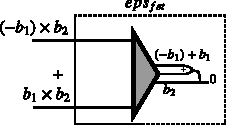
\includegraphics{diagrams/eps_fst.pdf}
}
\end{center}

The isomorphism {{(-b1) * b2 <-> -(b1 * b2)}} can be constructed in
terms of {{eps_{fst} }} as shown below. 

\begin{center}
\scalebox{0.9}{
  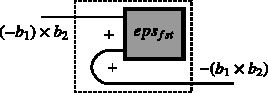
\includegraphics{diagrams/mult_neg.pdf}
}
\end{center}  

The second isomorphism can be built in the same way by merely swapping
the arguments. 

\paragraph*{Multiplying Negatives.}

{{b1 * b2 <-> (-b1)*(-b2)}}

This isomorphism is a consequence of the fact that $-$ is an involution: it
corresponds to the algebraic manipulation:

%% %subcode{opsem} include main
%% %! columnStyle = rc
%% %   & b1 * b2
%% % = & -(-(b1*b2)) 
%% % = & -((-b1)*b2)
%% % = & (-b1)*(-b2)

{{b1 * b2 = -(-(b1*b2)) = -((-b1)*b2) = (-b1)*(-b2)}}

\paragraph*{Multiplying and Adding Fractions.}
An isomorphism witnessing:

{{b1/b2 * b3/b4 <-> (b1*b3)/(b2*b4)}}

is straightforward. More surprisingly, it is also possible to construct
isomorphisms witnessing:

{{b1/b + b2/b <-> (b1+b2)/b}}

{{b1/b2 + b3/b4 <-> (b1*b4+b3*b2)/(b2*b4) }}


%%%%%%%%%%%%%%%%%%%%%%%%%%%%%%%%%%%%
\section{Two Dualities of Computation}
\label{sub:hof}

Information Effects, Filinksi, De Morgan

\subsection{Function Spaces}

Although these constructions are also standard, they are less known and they
are particularly important in our context: we devote a little more time to
explain them. Our discussion is mostly based on Abramsky and Coecke's article
on categorical quantum mechanics~\cite{abramsky-2008}.

In a compact closed category, each morphism {{f : b1 <-> b2 }} can be given a
\emph{name} and a \emph{coname}. For the additive fragment, the name
$\fname{f}$ has type {{0 <-> (-b1 + b2)}} and the coname $\fconame{f}$ has type
{{b1 + (-b2) <-> 0}}. For the multiplicative fragment, the name $\fname{f}$ has
type {{1 <-> ((1/b1) * b2))}} and the coname $\fconame{f}$ has type 
{{(b1 * (1/b2)) <-> 1}}. Intuitively, this means that for each morphism, 
it is possible to construct, from ``nothing,'' an object in the category that 
denotes this morphism, and dually it is possible to eliminate this object.
The construction of the name and coname of {{c : b1 <-> b2}} in the additive case 
can be visualized as follows:

\begin{multicols}{2}
\begin{center}
  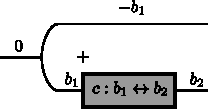
\includegraphics{diagrams/function.pdf}
\end{center}

\begin{center}
  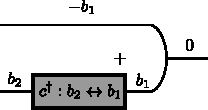
\includegraphics{diagrams/delimc.pdf}
\end{center}  
\end{multicols}

Intuitively the name consists of viewing {{c}} as a function and the coname
consists of viewing {{c}} as a delimited continuation.

In addition to being able to represent morphisms, it is possible to express
function composition. For the additive case, the composition is depicted
below:

\begin{multicols}{2}
\scalebox{1.1}{
    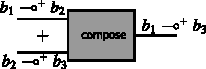
\includegraphics{diagrams/compose1.pdf}
}

\scalebox{0.8}{
    \includegraphics{diagrams/compose.pdf}
}
\end{multicols}
which is essentially equivalent to sequencing both the computation blocks as
shown below:

\begin{center}
  \includegraphics{diagrams/compose2.pdf}
\end{center}

Applying a function to an argument consists of making the argument flow
backwards to satisfy the demand of the function:
\begin{multicols}{2}
\begin{center}
\scalebox{1.0}{
  \includegraphics{diagrams/apply1.pdf}
}
\end{center}
\begin{center}
\scalebox{0.8}{
  \includegraphics{diagrams/apply2.pdf}
}
\end{center}
\end{multicols}

Having reviewed the representation of functions, we now discuss the
similarities and differences between the two notions of functions and their
relation to conventional (linear) functions which mix additive and
multiplicative components. For that purpose, we use a small example.
Consider a datatype {{color = R|Gr|B}}, and let us consider the following
manipulations:
\begin{itemize}
\item Using the fact that {{1}} is the multiplicative unit, generate
  from the input {{()}} the value {{((),())}} of type {{1 * 1}};
\item Apply the isomorphism {{1 <-> (1/b) * b}} in parallel to each of
  the components of the above tuple. The resulting value is
  {{((1/alpha1,alpha1),(1/alpha2,alpha2))}} where {{alpha1}} and
  {{alpha2}} are fresh logic variables;
\item Using the fact that {{*}} is associative and commutative, we can
  rearrange the above tuple to produce the value:

{{((1/alpha1,alpha2),(1/alpha2,alpha1))}}.

\end{itemize}

At this point we have constructed a strange mix of two {{b-o*b}} functions;
inputs of one function manifest themselves as outputs of the other. If
{{(1/alpha1,alpha2)}} is held by one subcomputation and {{(1/alpha2,alpha1)}}
is held by another subcomputation, these remixed functions form a
communication channel between the two concurrent subcomputations. Unifying
{{1/alpha1}} with {{color}} {{R}} in one subcomputation, fixes {{alpha1}} to
be {{R}} in the other. The type {{b}} thus takes the role of the type of the
communication channel, indicating how much information can be communicated
between the two subcomputations.  Depending on the choice of the type {{b}},
an arbitrary number of bits may be communicated.

Dually, the additive reading of the above manipulations correspond to
functions of the form {{b-o+b}}, witnessing isomorphisms of the form
{{0<->(-b)+b}}). The remixed additive functions express control flow transfer
between two subcomputations, \emph{only one of which exists} at any point,
i.e., they capture the essence of coroutines. 

It should be evident that in a universe in which information is not
guaranteed to be preserved by the computational infrastructure, the above
slicing and dicing of functions would make no sense. But linearity is not
sufficient: one must also recognize that the additive and multiplicative
spaces are different. 



%%%%%%%%%%%%%%%%%%%%%%%%%%%%%%%%%%%%%%%%%%%%%%%%%%%%%%%%%%%%%%%%%%%%%%%%%%%%%%%%
\section{Related Work} 
\label{sec:related}

The idea of ``negative types'' has appeared many times in the literature and
has often been related to some form of continuations. Fractional types are
less common but have also appeared in relation to parsing natural
languages. Although each of these previous occurrences of negative and
fractional types is somewhat related to our work, our results are
substantially different. To clarify this point, we start by reviewing the
salient point of the major pieces of related work and conclude this section
with a summary contrasting our approach to previous work.

\paragraph*{Declarative Continuations.} 
In his Masters thesis~\cite{Filinski:1989:DCI:648332.755574}, Filinski
proposes that continuations are a \emph{declarative} concept. He,
furthermore, introduces a symmetric extension of the $\lambda$-calculus in
which call-by-value is dual to call-by-name and values are dual to
continuations. In more detail, the symmetric calculus contains a ``value''
fragment and a ``continuation'' fragment which are mirror images. Pairs and
sums are treated as duals in the sense that the ``value'' fragment includes
pairs whose mirror image in the ``continuation'' fragment are sums. In
contrast, our language includes pairs and sums in the value fragment and two
symmetries: one that maps the pairs to fractions and another that maps the
sums to subtractions.

\paragraph*{The Duality of Computation.}
The duality between call-by-name and call-by-value was further investigated
by Selinger using control
categories~\cite{Selinger:2001:CCD:966910.966911}. Curien and
Herbelin~\cite{Curien:2000} also introduce a calculus that exhibits
symmetries between values and continuations and between call-by-value and
call-by-name. The calculus includes the type $A-B$ which is the dual of
implication, i.e., a value of type $A-B$ is a context expecting a function of
type $A \rightarrow B$. Alternatively a value of type $A-B$ is also explained
as a \emph{pair} consisting of a value of type $A$ and a continuation of type
$B$. This is to be contrasted with our interpretation of a value of that type
as \emph{either} a value of $A$ or a demand for a value of type $B$. This
calculus was further analyzed and extended by
Wadler~\cite{Wadler:2003,DBLP:conf/rta/Wadler05}. The extension gives no
interpretation to the subtraction connective and like the original symmetric
calculus of Filinski, introduces a duality that relates sums to products and
vice-versa.

\paragraph*{Subtractive Logic.} 
Rauszer~\cite{springerlink:10.1007/BF02120864,rauszer,rauszer2} introduced a
logic which contains a dual to implication. Her work has been distilled in
the form of \emph{subtractive logic}~\cite{Crolard01} which has recently been
related to coroutines~\cite{Crolard01082004} and delimited
continuations~\cite{Ariola:2009:TFD:1743339.1743381}.  In more detail,
Crolard explains the type $A-B$ as the type of \emph{coroutines} with a local
environment of type $A$ and a continuation of type $B$. The description is
complicated by what is essentially the desire to enforce linearity
constraints so that coroutines cannot access the local environment of other
coroutines. 

\paragraph*{Negation in Classical Linear Logic} 
Filinski~\cite{Filinski92} uses the negative types of linear logic to model
continuations. Reddy~\cite{Reddy91} generalizes this idea by interpreting the
negative types of linear logic as \emph{acceptors}, which are like
continuations in the sense that they take an input and return no
output. Acceptors however are also similar in flavor to logic variables:
they can be created and instantiated later once their context of use is
determined. Although a formal connection is lacking, it is clear that, at an
intuitive level, acceptors are entities that combine elements of our negative
and fractional types.

\paragraph*{The Lambek-Grishin Calculus.} The ``parsing-as-deduction'' style
of linguistic analysis uses the Lambek-Grishin calculus with the following
types: product, left division, right division, sum, right difference, and
left difference~\cite{Bernardi:2010:CSL:1749618.1749689}. The division and
difference types are similar to our types but because the calculus lacks
commutativity and associativity and only has limited notions of
distributivity, each connective needs a left and right version. The
Lambek-Grishin exhibits two notions of symmetry but they are unrelated to our
notions. In particular, the first notion of symmetry expresses commutativity
and the second relates products to sums and divisions to subtractions. In
contrast, our two symmetries relate sums to subtractions and products to
divisions.

\paragraph*{Our Approach.} The salient aspects of our approach are the
following:
\begin{itemize}
\item Negative and fractional types have an elementary and familiar
  interpretation borrowed from the algebra of rational numbers. One can write
  any algebraic identity that is valid for the rational numbers and interpret
  it as an isomorphism with a clear computational interpretation: negative
  values flow backwards and fractional values represent constraints on the
  context. None of the systems above has such a natural interpretation of
  negative and fractional types.
\item Because we are \emph{not} in the context of the full
  $\lambda$-calculus, which allows arbitrary duplication and erasure of
  information, values of negative and fractional types are first-class values
  that can flow anywhere. The information-preserving computational
  infrastructure guarantees that, in a complete program, every negative
  demand will be satisfied exactly once, and every constraint imposed by a
  fractional value will also be satisfied exactly once. This property is
  shared with systems that are based on linear logic; other systems must
  impose ad hoc constraints to ensure negative and fractional values are used
  exactly once.
\item In contrast to all the work that takes continuations as primitive
  entities of negative types, we view continuations as a derived notion that
  combines a demand for a value with constraints on how this value will be
  used to proceed with the evaluation (to the closest delimiter or to the end
  of the program). In other words, we view a continuation as a non-elementary
  notion that combines the negative types to demand a value and the
  fractional types to explain how this value will be used to continue the
  evaluation. As a consequence, the previously observed duality between
  values and continuations can be teased into two dualities: a duality
  between values flowing in one direction or the other and a duality between
  aggregate values composing and decomposing into smaller values. Arguably
  each of the dualities is more natural than a duality that maps regular
  values to a conflated notion of negative and fractional types, and hence
  requires notions like ``additive pairs'' and ``multiplicative sums.''
\end{itemize}

%%%%%%%%%%%%%%%%%%%%%%%%%%%%%%%%%%%%%%%%%%%%%%%%%%%%%%%%%%%%%%%%%%%%%%%%%%%%%%%%
\section{Conclusion and Future Work}
\label{sec:conc}

We have extended the language {{Pi}} that expressed computation
in the commutative semiring of whole numbers to {{PiEE}} that
expresses computation in the field of rationals.  Every algebraic
identity that holds for the rational numbers corresponds to a type
isomorphism with a computational interpretation in our model. We have
examined the two function spaces that arise in this model and
developed non-trivial constructions such as a SAT-solver that relies
on a multiplicative trace.

In another sense however, this paper is about the nature of duality in
computation. 
% The concept of duality is deep and significant and in many cases ---
% probably most famously in the divide between classical and intuitionistic
% mathematics --- contain non-trivial assumptions about our worldview.  The
% problem of duality in computation and logic, has many facets of which
% `continuation' and `higher order functions' are only one.
The concept of duality is deep and significant: we have opened the
door for us to consider, not one but two notions of
duality. Surprisingly this makes things substantially simpler. In
particular, instead of conflating pairs as dual to sums, the tradition
in mathematics has long been to consider fields with two notions of
duality: one for sums and one for pairs. This double notion of duality
has a crisp semantics, clear computational interpretation, and an
information theoretic basis.

Our work has barely scratched the surface of an area of computing which has
been explored in depth before but without the combined reversible
information-preserving framework and the two notions of duality. The new
insights point to further new areas of investigation, of which we mention
the three most significant ones (in our opinion).

%% \paragraph*{Int Construction} How are we preserving two compact
%% closed structures -- what does this imply about the Int
%% construction.

\paragraph*{Geometry of Interaction (GoI).}
Geometry of Interaction was developed by Girard~\cite{girard1989geometry} as part of
the development of linear logic. It was given a computational interpretation
by Abramsky and Jagadeesan~\cite{Abramsky:1994:NFG:184662.184664}, and was
developed into a reversible model of computing by
Mackie~\cite{Mackie2011,DBLP:conf/popl/Mackie95}. Preliminary investigations
suggest that many of the GoI machine constructions can be simulated in
{{PiEE}} by treating Mackie's bi-directional wires as pairs of wires in
{{PiEE}} and replacing the machine's global state with a typed value on
the wire that captures the appropriate state. This connection is exciting
because when viewed through a Curry-Howard lens it suggests that the logical
interpretation of {{PiEE}} would be a linear-like logic with a notion of
resource preservation and with a natural computational interpretation. 

\paragraph*{Computing in the Field of Algebraic Numbers.}
\label{sec:algebraic-field}
Algebraically, the move from {{Pi}} to {{PiEE}} corresponds to a
move from a ring-like structure to a full field. Our language {{PiEE}}
captures the structure of one particular field: that of the rational
numbers. As we have seen, computation in this field is quite expressive and
interesting and yet, it has two fundamental limitations. First it cannot
express any recursive type, and second it cannot express any datatype
definitions. We believe these to be two orthogonal extensions: recursive
types were considered in our previous paper~\cite{infeffects}; arbitrary
datatypes are however even more exciting that plain rationals as each
datatype definition can be viewed as a polynomial (see below) which
essentially means that we start computing in the field of algebraic numbers,
which includes square roots and imaginary numbers. As crazy as it might seem,
the type $\sqrt{2}$ and even the type $(1/2)+i(\sqrt{3}/2)$ ``make sense.''
In fact the latter type is the solution to the polynomial {{x^2-x+1=0}} which
if re-arranged looks like {{x=1+x*x}} and perhaps more familiarly as the
datatype of binary trees {{@@x.(1+x*x)}}. These types happen to have been
studied extensively following a paper by Blass~\cite{seventrees} which used
the above datatype of trees to infer an isomorphism between seven binary
trees and one!

We have confirmed that we can extended {{PiEE}} with the datatype
declaration for binary trees and build a witness for this isomorphism
that works as expected. However not every isomorphism constructed from
algebraic manipulation is computationally meaningful. To understand the
issue in more detail, consider the following algebraically valid proof
of the isomorphism in question:
\[\begin{array}{rclclclcl}
x^3 &=& x^2 x &=& (x-1) x &=& x^2 - x &=& -1 \\
x^6 &=& 1 \\
x^7 &=& x^6 x &=& x
\end{array}\]
The question is why such an algebraic manipulation makes sense type
theoretically, even though the intermediate step asking for an isomorphism
between $x^6$ and $1$ has no computational context. In the setting of
{{PiEE}}, this isomorphism can be constructed but it diverges on all
inputs (in both ways). This suggests that, in the field of algebraic numbers,
some algebraic manipulations are somehow 
``more constructive'' than others.

A related issue is that not all meaningful recursive types are
meaningful polynomials. For instance {{nat=@@x.(1+x)}} implies the
polynomial {{x=1+x}} which has no algebraic solutions without appeal
to more complex structures with limits etc. 

%% or dually that {{PiEE}} with recursive types
%%somehow lacks the ability to express all computations that are otherwise
%%algebraically meaningful.

% \begin{itemize}
% \item Maybe the problem is that there is cancellation in the second
%   case and cancellation with recursive types is problematic. However
%   not all cancellation is. So what gives?

% \item One idea is that irrationals correspond to an infinite amount of
%   computational work. If what we are cancelling is not the same
%   infinity, then things go wrong. 

% \item Chaitin has already shown that reals have inifite amount of
%   information which is paradoxical and problematic. This is a
%   different issue from that of the rational being infinite
%   computations.

% \item Finally, not all meaningful types are meaningful polynomials --
%   ex. nat. So this is not the whole story. 

% \end{itemize}

\paragraph*{Quantum Computing.} 
One understanding of quantum computing is that it exploits the laws of physics
to build faster machines (perhaps). Another more foundational understanding
is that it provides a computational interpretation of physics, and in
particular directly addresses the question of interpretation of quantum
mechanics. In a little known document, Rozas~\cite{Rozas:1987:CMO:889539}
uses continuations to implement the transactional interpretation of quantum
mechanics~\cite{transactional} which includes as its main ingredient a
fixpoint calculation between waves or particles traveling forwards and
backwards in time. Our work sheds no light on whether this interpretation is
the ``right one'' but it is interesting that we can directly realize it using
the primitives of {{PiEE}}. 

% A \emph{time
%   traveling} intuition is also applicable here.  In a normal cicruit, as
% computational steps are taken values flow from left to right,
% i.e. computational time progresses from left to right.  The action of
% {{eps+}} causes values, aka information particles, to flow from right to left
% i.e. backwards in computational time.  The interesting thing about this
% interpretation is that particles that travel backwards in time get to see and
% interact with the history of particles that they coexist with. This gives us
% an intuitive interpretation of the isomorphism {{(-b1)*b2<->-(b1*b2)}} (see
% Sec. \ref{sec:specific-constructions}) where it would otherwise seem that
% {{-b1}} and {{b2}} move in opposite directions. The backward flow of the
% {{-b1}} allows it to `see the past' of {{b2}} and is thus equivalent to both
% particles moving backward in time.

The multiplicative structure of {{PiEE}} also has a direct
connection to entangled quantum particles, or perhaps entangled
particles and anti-particles.  The idea of entanglement, that an
action on one particle is ``instantaneously'' communicated to the
other, is analogous to how unifying one value affects its dual pair
which is possibly in another part of the computation.  Again our model
sheds no light on whether this is related to how nature computes but
it is again interesting that we can directly realize the idea using
the primitives of {{PiEE}}.

% natural An analogy
% inspired by quantum mechanics is also applicable here.  The operator {{eta*}}
% is a site of fission that creates \emph{an entangled particle and
%   anti-particle}. These particles can be thought to be in a
% \emph{superposition} of states determined by their type. Both flow in the
% same direction in time.  In each possible world that the particle exists, it
% takes on a specific value inhibiting its type and correspondingly its
% entangled anti-particle takes the dual of the specific value. Since the
% particles are entangled, actions on one (such as transformation by
% application of an isomorphism) affects the other in much the same sense as
% \emph{action at a distance}. The `{{a-o*b}}' functions mentioned in the
% introduction, are first-class values and they correspond to these entagled
% pairs. Finally {{eps*}} operations are sites where corresponding particle and
% anti-particles annihilate each other. While appealing as an analogy, this
% description does not imply (or preclude) any formal connection with Physics.

% Are constructions are very similar to those developed in the context
% of QC. Is this how nature computes? Are the analogies to time
% traveling particles and anti-particles more concrete in some way? 

\begin{comment}
  
--- END -- 


%% \begin{center}
%%   \includegraphics{diagrams/dispatch.pdf}
%% \end{center}

% \subsection{Other}

%% To summarize negative, fractional, square root, and imaginary types all make
%% sense. What they help you accomplish as a programmer is to disassociate
%% global invariants into local ones that can be satisfied independently by
%% subcomputations with no synchronization or communication. A computation
%% producing something of type $a/b$ does not need to concern itself with who is
%% going to supply the missing $b$: it just does its part. Conversely faced with
%% a complicated task, a computation might decide to break it into pieces and
%% demand these pieces using negative types. 

%% It is no surprise that these types are closely related to quantum mechanics
%% and that they give us the feel that this is how nature computes. This is
%% speculation however.

%% In any case, in a framework where information can be copied and deleted, none
%% of this makes much sense. It is critical that these constraints and demands
%% can neither be duplicated nor erased.  This gives us the maximum
%% ``parallelism'' possible.


%% Say we have not considered recursion in this paper.

%% The simplest way to connect the In a conventional computational model, one
%% might realize this situation by simply writing the identity function: the
%% buyer hands the money to the seller to finish the transaction. The above
%% sequence of isomorphisms implements this identity function in a much more
%% interesting way, however.  of the above series of

%% On the producer side, the debt is paid for by the money computation with the
%% identity function. the producer and consumer must somehow share an explicit
%% dependency that allows the value. However in our model, the presence of
%% negative types allows the produced value to satisfy the demand without the
%% producer or consumer even knowing about each other. As is explained in detail
%% in

%% Furthermore, we illustrate their true appeal and expressiveness is brought
%% forth by viewing them in the context of an information-preserving
%% computational model.

%% In addition, we show how these types enrich our computational model, they
%% obey the same laws as the rational numbers. 


%% Specifically, isomorphisms enrich our computational model with have an
%% interesting computational interpretation

In particular, linear logic~\cite{Girard87tcs}, among other contributions,
exposed an additive/multiplicative distinction in logical connectives and
rules. In particular, linear logic includes additive disjunctions $\oplus$
and conjunctions $\with$ as well as multiplicative disjunctions $\parr$ and
conjunctions $\otimes$. Duality is also prominent in linear logic: it relates
the additive connectives to each other (the dual of $\oplus$ is $\with$ and
vice-versa) and the multiplicative connectives to each other (the dual of
$\otimes$ is $\parr$ and vice-versa).

%% We furthermore demonstrate that, in our model,
%% programming with these negative and fractional types, is a new ``revolution''
%% breaking dependencies...

Since Filinski, we've had the
idea that values and continuations are like mirror images. In a conventional
language, the negative (continuation) side is implicit and we introduce
information effects on the positive. Trying to recover the duality from this
distorted positive side has always been messy. Now it looks clean because we
have kept the positive side pure.

Continuations made their introduction to the world of programming language
semantics as a mathematical device to model first-class labels and
jumps~\cite{springerlink:10.1023/A:1010026413531}. In a remarkable
development, Filinski~\cite{Filinski:1989:DCI:648332.755574} observed that
--- with the right perspective --- this highly imperative concept was
actually the symmetric dual of values. The heart of the observation is that
values represent entities that flow from producers to consumers while
continuations represent \emph{demands} for such entities, that flow from
consumers to producers. In more detail, Filinski describes continuations as
representing ``the \emph{lack} or \emph{absence} of a value, just as having a
negative amount of money represents a debt.'' He then proceeds to construct a
language where values and continuations are treated truly symmetrically. To
that end, he abandons the $\lambda$-calculus amalgamation of functions and
values and distinguishes between three different syntactic classes:
functions, values, and continuations, with the property that any function can
be used either as a value transformer or as a continuation transformer.

This highly intuitive and appealing idea was further explored and refined by
many authors~\cite{Griffin:1989:FNC:96709.96714, Curien:2000,
  Wadler:2003, DBLP:conf/rta/Wadler05}. Yet, despite its appeal, the duality
between values and continuations 

%% Computationally, symmetry exhibits itself as a duality between two concepts.

%% Symmetry is pervasive in both natural and man-made environments. 

In 1989, Filinski~\cite{Filinski:1989:DCI:648332.755574} observed that values
and continuations are dual notions. This observation was followed by numerous

%% We introduced this thesis that computation should be based on isomorphisms
%% that preserve information~\cite{infeffects}. Since Filinski, we've had the
%% idea that values and continuations are like mirror images. In a conventional
%% language, the negative (continuation) side is implicit and we introduce
%% information effects on the positive. Trying to recover the duality from this
%% distorted positive side has always been messy. Now it looks clean because we
%% have kept the positive side pure.

%% In a technical sense, this paper extends the language of isomorphisms
%% {{Pi}}, with duality. Unlike Linear logic \cite{Girard87tcs} and
%% other systems which have one notion of duality over additive and
%% multiplicative components, {{PiEE}} has two notions of duality
%% -- an additive duality over the monoid {{(0, +)}} and a multiplicative
%% duality over the monoid {{(1, *)}}. Each axis of duality also give us
%% a function space and hence {{PiEE}} has an additive function
%% space corresponding to a notion of control or backtracking and a
%% multiplicative function space corresponding to a notion of unification
%% or constraint satisfaction.

The world of computation we are describing has:
\begin{itemize}
\item suppliers, 
\item consumers, and
\item bi-directional transformations
\end{itemize}
This is the same world described by the papers on the duality of computation
but that work only scratched the surface! We have the following features:
\begin{itemize}
\item we can start from the supplier and push the values towards the
  consumer (call-by-value in the duality of computation papers)
\item we can start from the consumer and pull the values from the suppliers
  (call-by-name in the duality of computation papers)
\item we can combine the pushing and pulling and values using eta/epsilon for
  sum types; these allow us to at any point in the middle of the computation
  create out of nothing a value to send to the consumers and a demand to send
  to the suppliers.
\item we can break a big data structure into fragments described by
  fractional types; the suppliers and consumers can produce and consume the
  pieces completely independently of each other. Eventually the pieces will
  fit together at the consumer to produce the desired output.
\item we can break a bi-directional transformation into pieces using square
  roots
\item we can take into account that values have phase (complex numbers),
  i.e., it is not that they flow towards the consumer or just towards the
  suppliers; they can be flowing in direction that ``30 degrees'' towards the
  consumer for example.
\end{itemize}

%% So it is all about breaking dependencies in some sense to allow for maximum
%% autonomy (parallelism) of subcomputations. It is probably the case that to
%% make full use of square root types and imaginary types, we have to move to a
%% vector space. If that's the case, we should probably leave this stuff out and
%% focus on negative and fractional types and only have a short discussion of
%% the polynomials restricted to seven trees in one and similar issues.

%% The conventional idea is to divide the world into a ``real'' one and a
%% ``virtual'' one. In the ``real'' world, we can define datatypes like
%% \verb|t=t^2+1| but we don't have additive inverses so it makes no sense to
%% talk of negative types and we can't rearrange the terms in the datatype
%% definition. However the observation is that we can map these datatypes to a
%% virtual world that has more structure (a ring that provides additive inverses
%% or a field that also provides multiplicative inverses) and then perform
%% computations in the ring/field. If we perform computations in the ring, then
%% some of these will use additive inverses in ways that cannot be mapped back
%% to the ``real'' world. Much of current research attempts to characterize
%% which computations done in the ring are valid isomorphisms between datatypes
%% in the ``real'' world. This is nice but is not what I am after. In fact I am
%% not interested in the ring or the semiring at all. I am interested in the
%% field and I want this field to be \textbf{the real world.} This is partly
%% motivated by the fact that Quantum Mechanics seems to demand an underlying
%% field and more generally that the field provides the maximum generality in
%% slicing and dicing computations. So assuming I live in a field and that the
%% negative, fractional, square root, and imaginary types are all ``real,'' how
%% do I compute in this field? Clearly there will be constraints on
%% ``measurement'' in the sense that a full program cannot produce any of the
%% crazy types but that's done outside the formalism in some sense just as in
%% Quantum Computing. The main question I am after is how to compute in this
%% field with first-class negative, fractional, etc. types. As I mentioned in my
%% previous email, we can produce programs that have types \verb|t^3 <-> -1| and
%% they ``run'' (but only to give infinite loops). 

%% So when a programmer writes the datatype declaration \verb|t = t^2+1|,
%% if we allow negative etc. then this is effectively writing
%% \verb|t = cubicroot{-1}|. If we are in the field then computations
%% that manipulate these trees can be sliced and diced even at interfaces
%% that expose the cubic root and the imaginary types.

%% Future work: develop a type system for a ``normal language'' that has
%% negative, fractional, etc. types as first-class types. More long term,
%% instead of adding one polynomial at a time, we can go to an algebraically
%% closed field. The complex numbers is an obvious choice but I would rather go
%% to something computable like the field of algebraic numbers. Is the adele
%% ring or the p-adics relevant here?


We show a deep symmetry between functions and delimited continuations, values
and continuations that arises in {{Pi}} in a manner that is reminiscent
of Filinski's Symmetric \lcal ~\cite{Filinski:1989:DCI:648332.755574}. The
symmetry arises by extending {{Pi}} with a notion of additive duality
over the monoid {{(+, 0)}} by including {{eta+}} and {{eps+}} operators of
Compact Closed Categories. The resulting dual types, which we denote {{-b}},
have a time traveling ``backward information flow'' interpretation and allow
for the encoding of higher-order function and iteration via the construction
of trace operators, thereby making the extended language {{PiEE}} a
Turing-complete reversible programming language with higher-order functions
and first-class delimited continuations.

%% We introduced this thesis that computation should be based on isomorphisms
%% that preserve information~\cite{infeffects}. Since Filinski, we've had the
%% idea that values and continuations are like mirror images. In a conventional
%% language, the negative (continuation) side is implicit and we introduce
%% information effects on the positive. Trying to recover the duality from this
%% distorted positive side has always been messy. Now it looks clean because we
%% have kept the positive side pure.

%% The way to think about something of type $A$ is that it is a value we have
%% produced. The way to think about something of type $-A$ is that is a value we
%% have already consumed. 

Other interpretations of the types of think about. The first one is
arithmetic obviously. Another one is languages consisting of sets of
string. The type 0 is the empty set, the type 1 is the set containing the
empty word, the $+$ constructor corresponds to union, and the $*$ constructor
corresponds to concatenation. The constructor $-$ would not correspond to set
difference however. It would correspond to marking the elements in the set as
``consumed'' so that if we take the union and a ``consumed'' element appears
in the other set, the two cancel. This makes it clear that concatenating a
produced $a$ and a consumed $b$ is not the same as concatenating a consumed
$a$ and a produced $b$. They really need to be kept separate. Incidentally,
division would be defined as follows:
\[
L_1 / L_2 = \{ x ~|~ xy \in L_1 \mbox{~for~some~} y \in L_2 \}
\]

Filinski proposes that continuations are a \emph{declarative} concept. He,
furthermore, introduces a symmetric extension of the $\lambda$-calculus in
which values and continuations are treated as opposites. This is essentially
what we are proposing with one fundamental difference: our underlying
language is not the $\lambda$-calculus but a language of pure isomorphisms in
which information is preserved. This shift of perspective enables us to
distill and generalize the duality of values and continuations: in
particular, in the conventional $\lambda$-calculus setting values and
continuations can be erased and duplicated which makes it difficult to
maintain the correspondence between a value and its negative counterpart.

The idea of using negative types to model information flowing backwards,
demand for values, continuations, etc. goes back to at Filinski's thesis. We
recall these connections below but we first note that all these systems are
complicated because in all these systems information can be ignored,
destroyed, or duplicated. Clearly the possibility of erasure of information
would mean that our credit card transaction is incorrect. In our work,
information is maintained and hence we have a guarantee that, in a closed
program, the debt must be accounted and paid for.

Much of previous work builds on the idea that there is one duality in
computation between values and continuations which manifests itself as a
duality between the call-by-value and call-by-name parameter-passing
mechanisms. The former mechanism focuses on evaluating expressions to values
even if these values are not demanded by the context; the latter focuses on
evaluating expressions to continuations even if these continuations might be
aborted. The idea that a continuation is dual to a value is intuitive but
then one would expect that the sum of two values naturally corresponds to the
sum of two continuations and that the product of two values naturally
corresponds to the product of two continuations.

check and say that our work teases the continuations into a negative part
(which simply demands a value) and a fractional part (which imposes
constraints on how this value will be used). So something like $-1/c$ is
needed to express a conventional continuation. Having two dualities makes the
whole calculus natural and symmetric.

Consider a continuation that takes $x$ and $y$ and swaps them. It can't be
expressed using two conventional continuations because the demand and the way
it is used are entangled together.

In accounts that are linear, the value and continuation that comprise the
subtractive type need to be constrained to ``stay together.'' This can be
achieved by various restrictions. In this work we have no such constraints,
the negative value can flow anywhere. The entire system guarantees that any
closed program would have to account for it. We don't have to introduce
special constraints to achieve that. Zeilberger in the paper on polarity and
the logic of delimited continuations uses polarized logic: he shows that if
positive and negative values are completely symmetric except that answer
types are positive, then the framework accommodates delimited
continuations. But he interprets negative values are control operators, or as
values defined by the shape of their continuations. We simply interpret
values of negative type as values flowing in the ``other'' direction.

This is essentially what we are proposing with one fundamental difference:
our underlying language is not the $\lambda$-calculus but a language of pure
isomorphisms in which information is preserved. This shift of perspective
enables us to distill and generalize the duality of values and continuations:
in particular, in the conventional $\lambda$-calculus setting values and
continuations can be erased and duplicated which makes it difficult to
maintain the correspondence between a value and its negative counterpart. In
contrast, in our setting, one can start from the empty type $0$, introduce a
positive value and its negative counterpart, and let each of these flow in
arbitrary ways. The entire framework guarantees that neither the value nor
its negative counterpart will be deleted or duplicated and hence that, in any
closed program, the ``debt'' corresponding to the negative value is paid off
exactly once. The forward and backward executions in our framework correspond
to call-by-value and call-by-name. This duality was observed by Filinski and
others following him but it is particularly clean in our framework.

\paragraph*{Logic Programming and Backtracking.} 
This is a constrained form of backtracking and a constrained form of
logic programming.

\paragraph*{Linear Logic and GoI.} 
Say something. 

\paragraph*{Int Construction.}
For a traced monoidal category {{C}} the Int construction produces a Compact
Closed Category called Int {{C}} \cite{joyal1996traced}.  Further we know
that the target of the Int construction is isomorphic to the target of \G
construction of Abramsky \cite{Abramsky96:0} from Haghverdi. However, note
that the {{PiEE}} is not the same as the image of the Int construction
on {{Pi0}}, since the later lacks a multiplicative tensor that
distributes over the additive tensor in Int {{Pi0}}.

once we combine the two structures, we seem to retain the monoidal
structure. How!?

\end{comment}

\acks We thank Jacques Carette for stimulating discussion, and Michael Adams,
Will Byrd, Lindsey Kuper, and Yin Wang for helpful comments and
questions. This project was partially funded by Indiana University's Office
of the Vice President for Research and the Office of the Vice Provost for
Research through its Faculty Research Support Program.  We also acknowledge
support from Indiana University's Institute for Advanced Study.

%%%%%%%%%%%%%%%%%%%%%%%%%%%%%%%%%%%%%%%%%%%%%%%%%%%%%%%%%%%%%%%%%%%%%%%%
\begin{small}
\bibliographystyle{abbrvnat}
\bibliography{cites}
\end{small}


\end{document}

%%%%%%%%%%%%%%%%%%%%%%%%%%%%%%%%%%%%%%%%%%%%%%%%%%%%%%%%%%%%%%%%%%%%%%%%
